
%%%%%%%%%%%%%%%%%%%%%      ConcordiaThesis.tex  -- MikTex 2.9     %%%%%%%%%%%%%%%%%
%%                                                                                                                  				
%%      A LaTex thesis template for ENCS graduate student from Concordia University (v2.0)                                  
%%                                                                                                                      				  
%%                  Last updated on Nov. 2, 2015                                                                         
%%         by     Suo Tan (tandysony@gmail.com)                                                                 
%%                   Design Lab, ENCS                                                                          				   
%%                   Concordia University                                                                       				    
%%                   Montreal, QC, CA                                                                           				     
%%                   July 15, 2015                                                                                				    
%%                                                                                                                      				    
%%  ---------------------------------------------------------------------------------------------------------------------------         
%%  This thesis template has been created to make it easy to prepare your thesis using         
%%  LaTeX while adhering to the Concordia University Thesis Specifications posted online:                           
%%  https://www.concordia.ca/artsci/english/programs/graduate/english-ma/thesis-deadlines-formatting.html#format
%%  http://www.concordia.ca/content/dam/concordia/offices/sgs/docs/handbooks/thesispreparationguide.pdf
%%
%%  The template has been tested with TeXstudio, TeXworks, CTex, and TeXnic                      
%%  under MikTex 2.9, with UTF-8 encoding.                                                                   
%%                                                                                                                                               
%%  The ConcordiaU.sty file MUST be included in your thesis folder.                                                     
%%                                                                                                                                                 
%%  If you are running it at your first time, make sure that you have internet connection. 			      
%%  You might need to download package(s) to ensure it works.											                         
%%  In case that you changed your reference database (*.bib file) and have any problem  	
%%  in generating references/citations correctly, please run in this sequence: "pdfLaTex  		
%%  -->  bibTex --> pdfLaTex".  This may help.                                                                                                    
%%                                                                                                                                                  
%%%%%%%%%%%%%%%%%% %%%%%%%%%%%%%%%% %%%%%%%%%%%%%%%%%%%%


%###################  BEGIN: Environment Setup  #######################

\documentclass[letterpaper,11pt,onecolumn,final]{report}              % define document type
\usepackage[left=1.5in,right=1in,top=1in,bottom=1in]{geometry}    % margin settings, required by Concordia University
\usepackage{ConcordiaU}                         % page maker definiation for Title Page, Signature Page, and styles customized for Concordia University 
\usepackage{setspace}                             % manually configuration to spacing is needed.
\doublespacing                                         % double spaced, required by Concordia University
\usepackage[natbibapa]{apacite}			      % citation and bibliography package
\usepackage{amsmath}                            % equations/formulas
\usepackage[dvips]{graphicx}                    % to include images. For those who use .eps images. The option [dvips] must be there.
\graphicspath{{Figures/}}                           % all figures are put in the folder named "figures"
\usepackage{subfigure}                            % enable subfigures
\usepackage{multirow} 					 		  % multirow in a table cellcc
\usepackage{indentfirst}                           % add indent to the first line of each paragraph
\usepackage{algorithmicx, algpseudocode}  %  write algorithms in pseudo code in a uniform style
\usepackage{algorithm}                             % algorithm and pseudocode environment
\usepackage[colorlinks,linkcolor=blue,anchorcolor=blue,citecolor=blue,urlcolor=blue]{hyperref}    % blue color for all links, urls and citations 
\usepackage{enumitem}
\renewcommand{\labelenumi}{(\arabic{enumi})}		%  "(1)." style for enuminated items 
\renewcommand{\labelitemii}{$\circ$}  	% (o) for the second level bullet items
\usepackage[titletoc,title]{appendix}
%\usepackage[titletoc,title]{appendix}   	   % appedix styles
%\usepackage{epsfig}					           % eps figures 
%\usepackage{epstopdf}                           % eps to pdf print
%\usepackage{multirow} 					          % multirow in a table cell
% my added packages
\usepackage{balance}
\usepackage{tabularx}
\usepackage{makecell}

%###################  END: Environment Setup  #######################


%###################  BEGIN: Degree Infor  #######################
% A blank field will be set to its defualt value 

\author{Akbar Dehghani}    % your full name. Defaut: Suo Tan
\title{A quantitative comparison of Overlapping and Non-overlapping sliding windows for human activity recognition using inertial sensors}    % your thesis title
\mastersDegree{Master of Applied Science}  % For master's degree only, will be ignored if PhD.  Default: Master of Applied Science
%%% Following two lines are required for Ph.D. thesis. %%%
\titleOfPhDAuthor{Mr.}         % or Ms., Mrs., Miss, etc. (only for PhD's)
% \PhD                                    % Masters by default, if comment out this line
\program{Computer Science}  % program towards your degree. E.g., Mechanical Engineering, Quality System Engineering. Default: I.E.
\dept{Computer Science and Software Engineering}       % your department. Default:  Mechanical and Industrial Engineering
\chairOfDept{Martin D. Pugh}     % your department chair. default:  Martin D. Pugh, Chair of MIE (As of Oct 2015)
\deanOfENCS{Amir Asif}       % Dean of ENCS. Default:  Amir Asif, Dean of ENCS (As of Oct 2015)

%%%% Your Final Examining Committee Members %%%
\chairOfCommittee{Name of the Chair}
\examinerExternalOfCommittee{Name of External Examiner}
\examinerFirstOfCommittee{Name of Examiner One}
\examinerSecondOfCommittee{Name of Examiner Two} % for PhD student 
\principaladvisor{Emad Shihab}
%%Following two lines are required if you have a co-supervisor
\cosupervisor                    
\myCoSupervisor{Tristan Glatard}

%###################  End: Degree Infor  #######################


\begin{document}
	
%   ----------------------  CITATION  REMINDER ----------------------------
%       \citet{key}  	         ==>>     Jones et al. (1990)
%       \citep{key}  	        ==>>     (Jones et al., 1990)
%       \citep{key1,key2}  	==>>     (Jones et al., 1990; Smith, 1989)

%%%%%%%%%% Pages with Roman Numerals %%%%%%%%%
\begin{abstract}
	% Requiment from the University: (1) must be page ''iii''; (2) text not exceeding 250 words. 
The sliding window technique is widely used to segment inertial sensor signals, i.e., accelerometers and gyroscopes, for activity recognition. In this technique, the sensor signals are partitioned into fix-sized time windows which can be of two types: (1) non-overlapping windows, in which time windows do not intersect, and (2) overlapping windows, in which they do. There is a generalized idea about the positive impact of using overlapping sliding windows on the performance of recognition systems in Human Activity Recognition. 
In this paper, we analyze the impact of overlapping sliding windows on the performance of Human Activity Recognition systems with different evaluation techniques, namely subject-dependent cross validation and subject-independent cross validation. Our results show that the performance improvements regarding to overlapping windowing reported in the literature seem to be associated with the underlying limitations of subject-dependent cross validation. Furthermore, we do not observe any performance gain from the use of such technique in conjunction with subject-independent cross validation. We conclude that when using subject-independent cross validation,
non-overlapping sliding windows reach the same performance as sliding windows. This result has significant implications on the resource usage for training the human activity recognition systems.
                
\end{abstract}
\begin{acknowledgments}
  Text of acknowledgments.
\end{acknowledgments}

%%%%%%%%%% Body of Thesis %%%%%%%%%%%%%%%%
\chapter{Introduction} \label{chap:introdcution}
% Thanks to the importance of comprehension of human demands and necessities, evaluation of people's habits and daily activities has been an active research area during the last decades. Such understanding has many applications in different fields including security, virtual reality, sports training, and health care. For 
% instance, this information has been used to detect anomalous behaviors such as 
% falls~\citep{luvstrek2009fall,tamura2009wearable,bianchi2010barometric} and track movement-related 
% conditions in seniors~\citep{chen2014implementing}. 
This chapter includes an overview of the thesis, along with a description of the
challenges. A summary is also given on contributions that are brought forth into this
thesis.
\section{Research Problem and Scope}
The tremendous advances in microelectronics and computer systems during the past decades enable wearable and mobile devices with remarkable abilities which are transforming society at a rapid pace. Such abilities including high computational power, low cost, and small size have provided a context in which people interact with them as inseparable parts of their life which produces huge volumes of data. There exists an active research area named \emph{Ubiquitous Sensing} with the main goal of extracting
knowledge from the such data~\cite{perez2010g}. In particular, thanks to the importance of comprehension of human demands and necessities, \emph{human activity recognition} (HAR) has become a task of high interest among researchers. Such understanding has many applications in different fields including security, virtual reality, sports training, and especially health care. For 
instance, this information has been used to detect anomalous behaviors such as 
falls~\citep{luvstrek2009fall,tamura2009wearable,bianchi2010barometric} and track movement-related 
conditions in seniors~\citep{chen2014implementing}. Another example is recognizing human activities to promote healthier lifestyles by encouraging do exercise~\citep{lin2006fish,consolvo2008activity} and preventing unhealthy habits such as tobacco use or unwholesome food~\citep{sazonov2009automatic,sazonov2011rf}.      

The recognition of human activities has been approached in two different ways, namely using external and wearable sensors~\citep{lara2012survey}. In the external scenario, the sensors are fixed in prearranged points and the recognition depends on the interaction of users with the sensors and also being accessible to them. As for wearable sensing, however,  the sensors are attached to the user's body and consequently, recognition is invariant to user interaction and position respect to the sensors. In general, Wearable sensing has been proven to be the prevalent technology in HAR~\citep{banos2014window};  
 

A classic example of using external sensors to recognize human activities is intelligent homes~\citep{kasteren2010activity,tolstikov2011comparison,yang2011activity,sarkar2011gpars}. In these systems, sensors are placed in target objects (e.g. stove, fridge, washing machine, etc) and users should interact with them so that they can recognize user's activities. Another example of external sensing is using cameras to recognize human activities~\citep{turaga2008machine,candamo2009understanding,joseph2010framework,ahad2008human} which is especially suitable for security and gaming~\citep{shotton2011real}. In general, systems with external sensors are able to recognize fairly complex activities such as eating, taking a shower, washing dishes, etc~\citep{lara2012survey}. However, such systems have several issues including privacy, pervasiveness, complexity, and maintenance cost~\citep{lara2012survey} which motivate to use of wearable sensors in HAR.

Wearable fitness devices such as the Nike Fuel Band and Fit-Bit Flex are good examples for wearable sensing. These devices which can be used during exercise, track their wearers physical activities (e.g. number of steps taken) and caloric expenditure. Users may use such information to set their own fitness goals and monitor their progression. In general, the employed sensors in wearable devices can be categorized into three groups: (1) sensors to measure the user's movement (e.g. accelerometer, gyroscope, GPS, etc), (2) sensors to measure the environmental variables (e.g. temperature and humidity), and (3) sensors to measure the physiological signals (e.g., heart rate and electrocardiogram).      


Most HAR systems use an Activity 
Recognition Process (ARP) to detect activities. These systems usually consist of one or more sensors attached to different parts of a person's body that provide diverse streams of sensor data. Such data streams, subsequently, are segmented into several time windows with specific length and from which feature vectors are extracted and fed to a classifier. 

\section{Motivation behind this Research}
Segmentation in time windows is a critical process in ARP, often implemented with 
sliding windows ~\citep{janidarmian2017comprehensive,banos2014window} that can be of two types: (1) non-overlapping windows, in which time windows do not intersect, and (2) overlapping windows, in which they do~\citep{lara2012survey}.
Both overlapping and non-overlapping windows are commonly used in the literature. For instance, in Recofit~\citep{morris2014recofit}, sensor signals are windowed into 5-second overlapping windows sliding at 200ms. Another example is the work in~\citep{banos2014window}, that uses non-overlapping sliding windows to partition sensor signals. 
%However, it remains unclear which technique is the most relevant.

Several works~\citep{keogh2001online,janidarmian2014automated} have shown that using overlapping sliding windows instead of non-overlapping ones improves the accuracy of the recognition systems. However, the amount of such improvement and its sources in HAR remain unclear. This study addresses this question: based on a detailed, quantitative analysis of multiple datasets, we explain why and by how much overlapping windows affect the performance of ARP. We report and discuss the general and per activity impacts of these two methods considering two cross validation (CV) techniques namely subject-dependent CV and subject-independent CV. 

\section{Thesis Contributions}
The major contributions of the thesis are as follows:

\begin{itemize}

\item An in-depth investigation of how HAR system performance is impacted by overlapping and non-overlapping sliding windows.
\item An investigation of the main reasons of performance improvement by overlapping sliding windows in HAR systems 
\item A set of publicly available scripts\footnote{\url{http://www.github.com/big-data-lab-team/paper-generalizability-window-size}} to help the research community further shed light on the important topic of choosing the types of sliding windows in HAR.
\end{itemize}

\section{Thesis Overview}
\noindent\textbf{Chapter two - Background on Human Activity Recognition using Wearable sensors:}
Discusses the background of
HAR using wearable devices. This chapter is divided in two parts: 
\begin{itemize}
    \item \textbf{Part 1:}
    Describes the different stages of ARP and also the common used techniques in each stage. Moreover, this part explains and compares diverse types of sliding windows and also system evaluation techniques in HAR systems. \item \textbf{Part 2:}
    This part reviews the segmentation process using the sliding window technique in previous works in HAR fields. 
  
\end{itemize}{}
\noindent\textbf{Chapter three - Methodology:}
Explains the used datasets in this study and our ARP setting including window sizes, feature sets and classifiers.

\noindent\textbf{Chapter four - Results:}
Presents the results and conclusions of five different experiments where were conducted to investigate the general and per activity impacts of overlapping and non-overlapping sliding windows on HAR systems. For each experiment, setting, results and conclusion are presented.

\noindent\textbf{Chapter five - Discussion and conclusion:}
Discusses and compares the results of different experiments. Finally, we conclude the thesis by summarizing our work and findings and offering remarks on possible future works.   

 
        


        
\chapter{Background on Human Activity Recognition using Wearable sensors} \label{chap:background}
\section{Background }
In this section, we provide an overview of a typical activity recognition process, aka ARP, explain and compare different sliding windows techniques and describe common evaluation methods in HAR.
\subsection{Activity Recognition Process}\label{subsec:ARP}

\begin{figure}[ht]
    \centering
    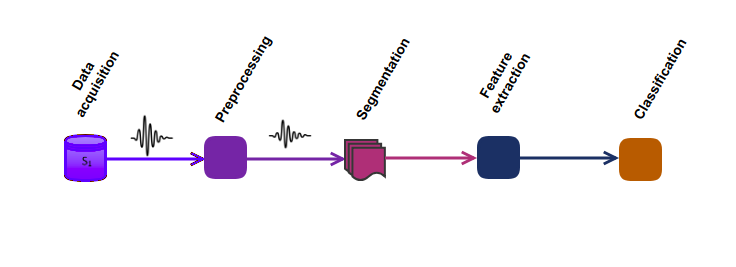
\includegraphics[width=1\textwidth]{Figures/HARP.png}
    \caption{Human activity recognition process}
    \label{fig:tsprocess}
\end{figure}

ARP is composed of a sequence of signal processing, pattern recognition, and 
machine learning techniques~\cite{bulling2014tutorial}. It mainly 
consists of 5 steps, shown in Figure \ref{fig:tsprocess} and 
explained hereafter.

\begin{figure}[ht]
    \centering
    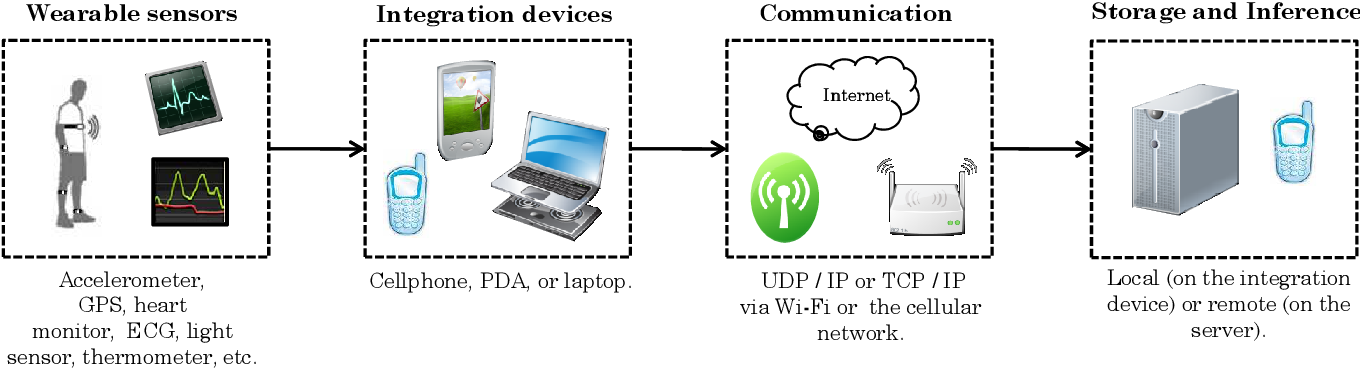
\includegraphics[width=.9\textwidth]{Figures/general_data_acqu.png}
    \caption{Generic data acquisition architecture for HAR extracted from~\cite{lara2012survey}}
    \label{fig:data_aqc}
\end{figure}

\subsubsection{Data acquisition} Several sensors are attached to different body parts. They mostly acquire 3D acceleration, gyroscopic and magnetic field measurements, etc, which measure different attributes such as  motion~\citep{iglesias2011ubiquitous}, location~\citep{choujaa2008tracme}, temperature~\citep{parkka2006activity}, and ECG~\citep{jatoba2008context}. Sensors discretize signals at a given frequency, typically 50Hz for 
daily activities or 200Hz for fast sports, and transmit data through UDP/IP or TCP/IP protocols to integration devices (ID) to be preprocessed~\citep{lara2012survey}. IDs can be different devices including cellphones, PDAs, laptops or a customized embedded systems~\citep{lara2012survey}. Figure~\ref{fig:data_aqc} shows a generic architecture of data acquisition in HAR. It should be noted that all of the mentioned components are not necessarily implemented in every HAR systems.      
 

\subsubsection{Preprocessing} Data points coming from sensors may
include artifacts of various origins such as 
electronic fluctuations, sensor malfunctions, and physical activities~\cite{bulling2014tutorial}. To eliminate such artifacts, filtering techniques are commonly applied, such as the Butterworth low-pass filter, which flats the coming signals as much as possible through rolling off down the higher frequencies beyond the cut-off point to zero ~\cite{morris2014recofit,selles2005automated,najafi2003ambulatory}. In any case, preprocessing techniques need to preserve
the signal characteristics that carry relevant information about the activities and consequently, they should be used with care as they may remove valuable information from the signals.


\subsubsection{Segmentation}
In this stage, the coming signals from sensors are partitioned into time windows labeled from the most frequent activity in the window. There are several ways to segment the sensor signals in HAR field which can be categorized into three groups, namely activity-defined windows, event-defined windows and sliding windows~\cite{banos2014window}. 

\noindent\textbf{Activity-defined windows}- In this technique, signals are partitioned based on the detection of activity changes, so the start and end points of each activity should be determined. Since the times of activities can be different, the window sizes are not fixed. In the literature, several methods have been used to identify the activity-transition points. For instance,~\citep{sekine2000classification,nyan2006classification} suggest a model based on the variations in the frequency characteristics to identify activity-transition points.  Another example is work in~\citep{yoshizawa2013parameter} which propose a heuristic method to separate static actions from dynamic ones. In the simpler scenario, the activity-transition points can be identified by user feedback~\citep{lester2006practical,he2009activity,figo2010preprocessing,dernbach2012simple}. 

\noindent\textbf{Event-defined windows}- Some activities such as meal preparation could be better recognized as a sequence of actions performed in a certain order. However, such activities are irregular and the order of actions for a specific one can be different and under such circumstances, the identification of specific events is particularly advised. The goal of event-defined windows is locating specific events in the signals to be used for data segmentation. In particular, this method is widely used in Gait analysis~\citep{banos2014window}. In this case, the models aim to detect heel strikes (the initial floor contact) and toe-offs (the end of floor contact) events. In the literature, several methods have been utilized to identify such events including analyzing the foot's linear acceleration~\citep{aminian1999temporal,selles2005automated}, Foot~\citep{aminian2002spatio} and shank~\citep{jasiewicz2006gait} sagittal angular velocity, using clustering models such as Gaussian mixture~\citep{aung2013automated}, using external mechanisms like stopwatch to register the first crossing time of hind foot and lead foot from a given start and end lines respectively~\citep{dobkin2011reliability}, etc. Identifying such events, subsequently can be used to recognize activities. For example,~\citep{benocci2010wearable} uses a model to recognize walking by identifying the gait cycle on a single foot tagged through a heel strike event. Like activity-defined windows, the window sizes are not fixed since the events may not be uniformly distributed in time.  

\begin{figure}[htp]
  \centering
  \subfigure[Non-overlapping]{
\label{subfig:NOSW}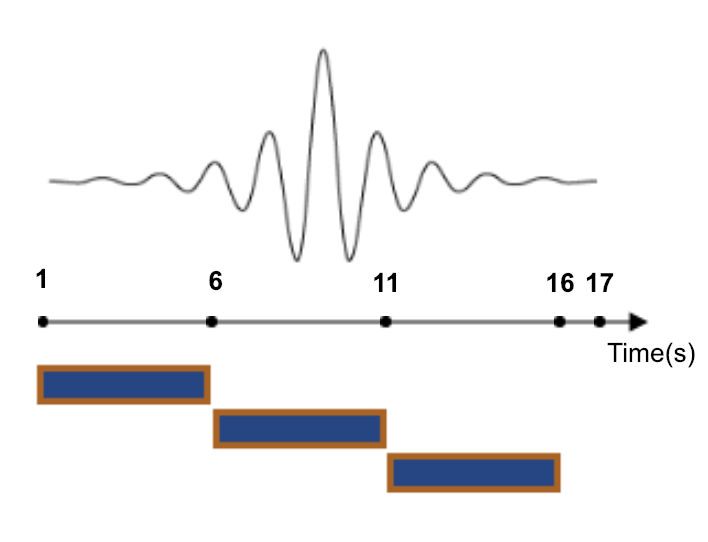
\includegraphics[scale=0.5]{Figures/NOSW.png}}\quad
  \subfigure[Overlapping-2 s sharing ]{\label{subfig:OSW}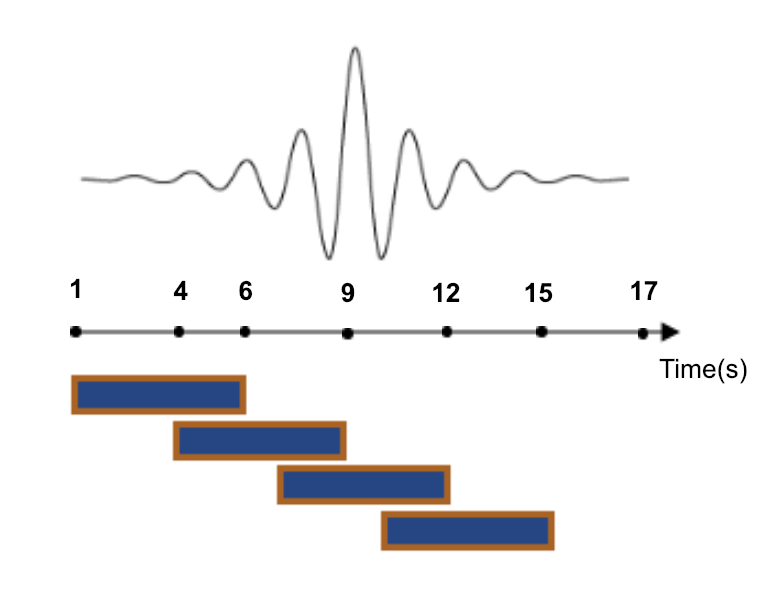
\includegraphics[scale=0.5]{Figures/OSW.png}}

   \caption{5-second sliding windows. }
   \label{fig:SlidingWindow}
\end{figure}

\noindent\textbf{Sliding windows-} The sliding window approach is the most widely used method in the segmentation step of ARP due to its implementational simplicity and lack of preprocessing~\citep{banos2014window}. In this approach, the sensor signals are split into windows of fixed size. If there is overlap between adjacent windows, this technique is known as overlapping sliding window, and if not, it is called non-overlapping windows technique. 
Figure~\ref{fig:SlidingWindow} illustrates the 
non-overlapping and overlapping windowing techniques.

\noindent\textbf{Formal definition-}
Mathematically, a sliding window process can be defined as follows.
Assume a stream of data values $x_i \in \mathbb{R} $ at times $t_i(i \in \mathbb{N})$. For simplicity, we assume that $t_0 = 0$ and the sampling period remains constant at $\Delta{T}$, i.e., 

$\forall i \in \mathbb{N}, t_{i + 1} - t_i = \Delta{T}$.

A fixed length sliding window splits the data stream into individual segments, where each segment
consists of n $(n \in \mathbb{N},n>1)$ samples. Consequently, the window size T in seconds is computed as follows:

$T = (n-1)\Delta{T}$,

where $\Delta{T}$ is the sampling period. We also denote $p \in {\{0,1,2,...,n-1\}}$ as the number of samples that are
within the overlapping period between two consecutive windows, where p = 0 refers to the
scenario with non-overlapping windows. Next, the overlapping period between two consecutive
windows in seconds, i.e., OP, can be computed as follows:

$OP = p\Delta{T}$.

Many research articles define the overlapping period as a percentage of the overall window length,
e.g., 80\% overlapping windows. The overlapping period in percentage can also be found as follows:

$ OP(\%) = \frac{p}{n} $

Finally, we can express each window/segment $S_k(k \in N)$ as a set of data values $x_i$ as follows:

$S_K = \{ x_{k(n-p)},x_{k(n-p)+1},..., x_{k(n-p)+n-1}\},(k \in \mathbb{N})$
\newline


There is a generalized idea that using overlapping sliding windows increases the performance of classifiers in HAR~\citep{janidarmian2014automated}, since they involve more data points, and unlike the non-overlapping windows, they are not prone to missing important events~\citep{coggeshall2005asset}, particularly within activity transition periods. While these assumptions are generally true, we will show later with our detailed experiments that non-overlapping windows overall deliver comparable recognition accuracy, while majorly reducing the required training computations and memory usage.
The number of data points in a time window, a.k.a the window size, heavily impacts the 
performance of the model~\citep{bulling2014tutorial,banos2014window}. Finding the optimal window size depends on the specific requirements of the HAR system. For instance, the number of activities for which system is devised or special recognition time~\citep{banos2014window}. However, in any case, the window size should be properly selected in such a way that each window contains enough samples (at least one cycle of an activity) to be differentiable from similar movements~\citep{janidarmian2017comprehensive}. The current method 
to select the window size is empirical~\citep{bulling2014tutorial}. We apply ARP with different window sizes which mostly selected from the values used in previous works, and choose the one which maximizes the performance of the recognition system. This process can be very time consuming due to the fact that there is no prior knowledge about the optimal window size and the entire space should be searched in an uninformed way. Table~\ref{tab:win_size_distribution} shows an extensive review of used window size in previous studies. 




\begin{table}[htp]
    \centering
\begin{tabular}{|c|>{\centering}m{10cm}|}
\hline 
Window size range (s) & publications\tabularnewline
\hline 
\hline 
0 - 1 & \citep{pirttikangas2006feature},~\citep{stikic2008adl},~\citep{marx2012ad},~\citep{huynh2005analyzing},~\citep{kern2003multi},~\citep{maurer2006activity},~\citep{suutala2007discriminative},~\citep{amft2008recognition},~\citep{han2010implementation},~\citep{wang2012real}\tabularnewline
\hline 
1 - 2 & \citep{pirttikangas2006feature},~\citep{stikic2008adl},~\citep{huynh2005analyzing},~\citep{sun2010activity},~\citep{gjoreski2011accelerometer}\tabularnewline
\hline 
2 - 3 & \citep{mannini2013activity},~\citep{stikic2008adl},~\citep{preece2008comparison},~\citep{mantyjarvi2001recognizing},~\citep{huynh2005analyzing},~\citep{wang2007accelerometry},~\citep{khan2010human},~\citep{sun2010activity},\citep{nam2013physical},\citep{nam2013child} \tabularnewline
\hline 
3 - 4 & \citep{sun2010activity}\tabularnewline
\hline 
4 - 5 & \citep{mannini2013activity},~\citep{stikic2008adl},~\citep{huynh2005analyzing},\citep{parkka2006activity},~\citep{sun2010activity}\tabularnewline
\hline 
5 - 6 & \citep{ravi2005activity},~\citep{altun2010human},~\citep{sun2010activity},~\citep{atallah2011sensor},~\citep{lee2011activity} \tabularnewline
\hline 
6 - 7 & \citep{bao2004activity},
~\citep{Huynh2007ScalableRO},
~\citep{sun2010activity},
~\citep{jiang2011method} \tabularnewline
\hline 
7+ & \citep{mannini2013activity},~\citep{stikic2008adl},~\citep{krause2003unsupervised},~\citep{parkka2006activity},~\citep{kwapisz2011activity},~\citep{siirtola2012user},~\citep{hemalatha2013frequent},~\citep{zheng2013physical} \tabularnewline
\hline 
\end{tabular}
    \caption{Distribution of the activity recognition research studies based on the utilized window size}
    \label{tab:win_size_distribution}
\end{table}


\subsubsection{Feature extraction}
\begin{table}[h]
    \centering
\begin{tabular}{|c|>{\centering}m{8cm}|>{\centering}m{4cm}|}
\hline 
Group & Methods& Publications\tabularnewline
\hline 
\hline 
Time domain & Mean, Standard deviation, Variance, Interquartile range, Mean absolute deviation, Correlation between axes, Kurtosis, Root Mean Square, Averaged derivatives, Skewness, Zero Crossing Rate, Mean Crossing Rate, Pairwise Correlation, Spectral Entropy & ~\citep{banos2014window},~\citep{morris2014recofit},
~\citep{parkka2006activity},~\citep{tapia2007real},
~\citep{kao2009development},~\citep{maurer2006activity},
~\citep{zhang2011feature} \tabularnewline
\hline 
Frequency domain & Fourier Transform, Discrete  Cosine
Transform &~\citep{bao2004activity},~\citep{morris2014recofit},~\citep{chen2008online},~\citep{altun2010human}\tabularnewline
\hline 
Others & Principal  Component  Analysis (PCA), Linear
Discriminant  Analysis (LDA), Autoregresive  Model
(AR), HAAR filters &~\citep{morris2014recofit},~\citep{altun2010human},~\citep{he2009activity},~\citep{chen2008online},~\citep{hanai2009haar}\tabularnewline
\hline 
\end{tabular}
    \caption{Summery of common used features in HAR publications }
    \label{tab:statistical_features}
\end{table}

\begin{figure}[h]
    \centering
    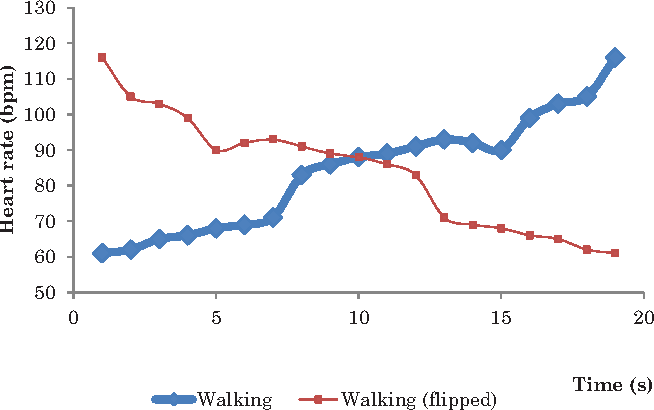
\includegraphics[width=.9\textwidth]{Figures/walking_heart.png}
    \caption{Heart rate signal for walking (bold) and flipped signal (thin) extracted from~\cite{lara2012survey}}
    \label{fig:walking_heart}
\end{figure}

\begin{table}[h]
    \centering
\begin{tabular}{|c|>{\centering}m{8cm}|>{\centering}m{5cm}|}
\hline 
Function & Equation & Parameters\tabularnewline
\hline 
Linear &  \begin{center}
      $F(t)= mt + b$
 \end{center} & \{m, b\}\tabularnewline
Polynomial & \begin{center}
      $F(t)= a_0 + {a_1}t+ ... + a_{n-1}t^{n-1}$ \end{center} & 
      $\{a_0, ..., a_{n-1}\}$ \tabularnewline
Exponential &  \begin{center}
      $F(t)= a{|b|}^t + c$
 \end{center}  &\{a, b, c\}\tabularnewline
Sinusoidal & \begin{center}
      $F(t)= a \times sin(t + b )+ c$
 \end{center} & \{a, b, c\} \tabularnewline
\hline 
\end{tabular}
    \caption{Common functions implemented by structure detectors extracted from~\cite{lara2012survey}}
    \label{tab:structure_features}
\end{table}




The main reason for applying feature extraction on each time window is that it is almost impossible for two given time windows to be exactly identical even if they come from the same subject doing the same activity~\citep{lara2012survey}. On the other words, through that we can filter out relevant information and obtain a quantitative measures of each time window which can further be used to compare with other time windows. In general, feature extraction methods can be categorized into two groups: statistical
and structural~\citep{article}. Regarding the statistical methods, they use quantitative characteristics of the data to extract features. Table~\ref{tab:statistical_features} shows a summery of common statistical features in HAR literature. As for structural methods, however, they consider the interrelationship among data to extract features from signals. In some situations, such features play an extremely significant role in HAR. To illustrate, consider Figure~\ref{fig:walking_heart} which represents the heart rate signal for a person that was walking and the same signal in reverse temporal order. Under such circumstances, statistical features such as time domain and frequency domain features are not discriminative since for these two signals, most of them are equal and we need to use utilize features that take the structure of signals into account. According to~\cite{lara2012survey} and from a mathematical perspective, given a time series $Y(t)$, a structure detector implements a function $f(Y(t)) = \hat{Y}(t)$ such that $\hat{Y}(t)$ approximates $Y(t)$. Table~\ref{tab:structure_features} shows the common functions implemented by structure detectors. In general, choosing the feature extraction method and feature sets are dependent to the nature of signal. For instance, acceleration signals tend to fluctuate and be oscillatory and the features extraction method should be able to handle the high variability of signals.


\subsubsection{Classification}

\begin{table}[h]
    \centering
\begin{tabular}{|c|>{\centering}m{8cm}|>{\centering}m{5cm}|}
\hline 
Classifier & Publications\tabularnewline
\hline 
\hline 
Decision tree &  ~\citep{banos2014window},~\citep{4650398},~\citep{inproceedings},~\citep{Bao2004ActivityRF},~\citep{4650199}\tabularnewline
\hline 
Naive Bayes &~\citep{banos2014window},~\citep{tapia2007real},~\citep{bao2004activity},~\citep{6181018},~\citep{kern2003multi},~\citep{ravi2005activity}\tabularnewline
\hline 
K-nearest neighbors &~\citep{banos2014window},~\citep{4650398},~\citep{inproceedings},~\citep{maurer2006activity},~\citep{ravi2005activity}\tabularnewline
\hline 
Neural Networks &~\citep{8767219},~\citep{al2019deep},~\citep{Wang2018DeepLF}\tabularnewline
\hline 
Support Vector Machines &~\citep{morris2014recofit},~\citep{4620779},~\citep{Wang2018DeepLF},~\citep{4761688},~\citep{Huynh2007ScalableRO},\citep{zhang2011feature}\tabularnewline
\hline 
Markov models &~\citep{Vinh:2011:SCR:2036609.2036624},~\citep{5152756}\tabularnewline
\hline 
Nearest Centroid Classifier &~\citep{huynh2005analyzing}\tabularnewline
\hline 
\end{tabular}
    \caption{Summery of common classifiers in HAR publications }
    \label{tab:classifiers}
\end{table}


Finally, a classifier is trained on the vector of extracted features and corresponding 
labels, and assigns future 
observations to one of the learned activities. Table~\ref{tab:classifiers} summarizes most common classifiers and some work examples of them in the HAR field.  


\subsection{System evaluation}
\label{sub:CVs}
One of the most important step in designing each system is evaluation. The evaluation in HAR has been mostly carried out through k-fold CV. In k-fold CV (Figure~\ref{fig:Shuffle-cv}), the overall data is randomly partitioned in $k$ equal subsets. The model is then trained on $k-1$ subsets, and the remaining one is used for testing~\citep{trevor2009elements}. In this process, the test set can be any part of the dataset meaning that training and test sets may contain the data of same subject and due to that, this method is referred to as subject-dependent CV in literature~\cite{al2019deep}.  
The main assumption of this process is that \emph{samples are Independent and Identically Distributed (i.i.d.)}~\cite{arlot2010survey}, which means that all the data points are sampled independently from the same distribution.  However, samples drawn from a given subject are likely to \emph{not} be independent, for two reasons. First, there is a strong inter-subject variability in the way activities are conducted~\cite{bulling2014tutorial}. This means that the similarity of samples drawn from the same subject is likely to be higher than that of samples drawn from different subjects. Several factors might explain such variability, including sex, gender, age or experience. Second, there is a temporal dependence between activities performed by the same subject: the similarity between samples drawn in a short time interval, for instance in the same training session in case of training activities, will most likely be higher than that of samples drawn further apart in time. This is due to factors such as fatigue and training. Thus, k-fold CV may overestimate the performance of recognizer systems in HAR. Such overestimation is even larger when k-fold CV is used with overlapping sliding windows since the overlap between adjacent windows is another source of dependency between data points. A more formal discussion about the problems of k-fold CV in HAR can be found in~\cite{dehghani2019subject}.   


To address these issues, the training and testing sets should be split by subject. In this method which is known as subject-independent CV~\cite{al2019deep,janidarmian2017comprehensive}, in each iteration the model is trained on all the subjects except one, which is used for testing. In this way, the intra-subject dependencies present in subject-dependent CV are hence removed. It should be noted that, in this case, as is shown in Figure~\ref{fig:Subjective-cv}, the number of folds is lower or equal to the number of subjects in the dataset.    


\begin{figure}[htp]
  \centering
  \subfigure[Subject-dependent CV]
  {\label{fig:Shuffle-cv}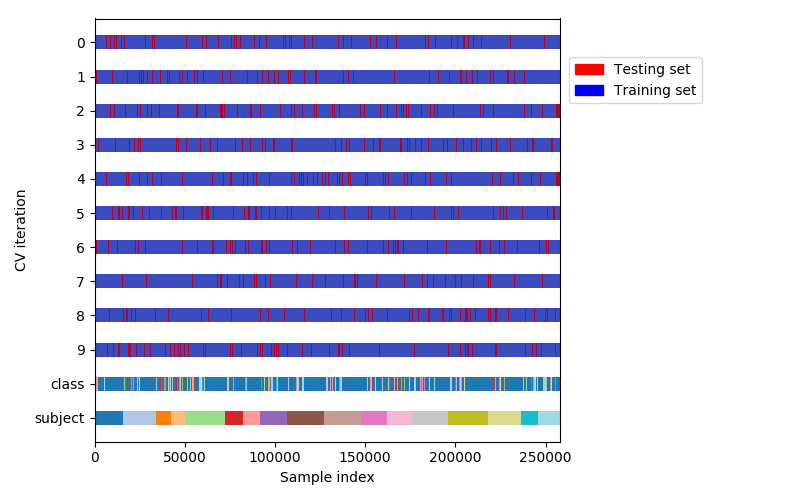
\includegraphics[scale=0.36]{Figures/ShuffleSplit.png}}\quad
  \subfigure[Subject independent CV]
  {\label{fig:Subjective-cv}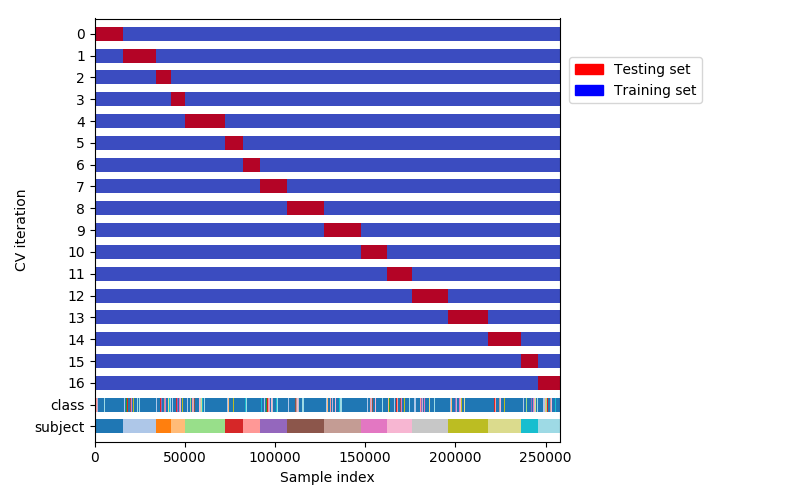
\includegraphics[scale=0.36]{Figures/LeaveOneGroupOut.png}}
   \caption{Different types of CV in HAR}
    \label{fig:CVs}
\end{figure}
\section{Related work}
The sliding window technique is widely employed in HAR, and the literature contains a plethora of examples where both, overlapping (e.g.,~\cite{bao2004activity,tapia2007real,lara2012centinela,morris2014recofit}) and non-overlapping time windows are used (e.g.,~\cite{minnen2007recognizing,reddy2010using,cheng2010active,banos2014window}).
\subsection{Overlapping sliding windows}

The work by Ling Bao and Stephen S. Intille~\cite{bao2004activity} uses overlapping sliding windows to segment signals coming from five biaxial accelerometers placed on 20 subjects (13 males and 7 females) under laboratory and semi-naturalistic conditions while performing 20 daily activities. Subsequently, each window is transformed into a set of features namely mean, energy,  frequency-domain entropy, and correlation of acceleration data. The authors use k-nearest neighbor (KNN), decision tree (DT), and naive bayes (NB) classifiers, and subject-independent cross-validation (CV) and subject-dependent CV for system evaluation. They reach the overall accuracy of 84\% with DT under the subject-independent CV process.

Another example is work by Tapia et al~\cite{tapia2007real} where the authors develop a real-time recognition system to recognize physical activities and in some cases, their intensities. They segment the signal data collected from 21 subjects wearing triaxial wireless accelerometers and a wireless heart rate monitor while performing 30 physical gymnasium activities using overlapping sliding windows. Subsequently, from each window, they extract time domain and frequency domain features and using a DT classifier they recognize activities.with an accuracy of 94.6\% using
subject-dependent CV and 56.3\% using subject-independent CV. 

Lara et al~\cite{lara2012centinela} combine acceleration data with vital signs to improve the performance of HAR systems. They apply ARP on a dataset which was collected from eight subjects (7 males and 1 female) while wearing a BioHarness™ BT chest sensor strap\footnote{\url{http://www.zephyr-technology.com/bioharness-bt.html}}. Using data from a triaxial accelerometer and vital signs, they detect five activities including running, walking, sitting, ascending, or descending. Sensor signals are partitioned into overlapping time windows with three different sizes: 5-seconds, 12-seconds, and 20-seconds sliding at 50\% of their sizes and 90 features were extracted from each time window. NB, DT, Bayesian Network, Multilayer Perceptron, Additive Logistic Regression and classifier ensembles are used to recognize activities. They achieve up to 95.7\% overall accuracy, which was evaluated through subject-dependent CV. Their results also indicate that vital signs are useful to discriminate between certain activities like running and sitting compared to the cases that utilize acceleration data only.


Recofit~\cite{morris2014recofit} is a well-known reference on HAR, which applies ARP on a dataset of accelerometer and gyroscope data collected from 114 participants over 146 sessions. The authors address three major challenges namely (1) 
segmenting exercise from intermittent non-exercise periods, (2) 
recognizing which exercise is being performed, and (3) counting repetitions. Data points are windowed into 5-second overlapping windows sliding at 200 ms and subsequently, each window is transformed into 224 features. Linear support vector 
machines (SVM) are used in the classification stage and evaluated by 
subject-independent CV. Spectacular performance is achieved, with precision and 
recall greater than 95\% to identify exercise periods, recognition 
of up to 99\% for circuits of 4 exercises, and counting  
accurate to $\pm$1 repetition, 93\% of the time.


\subsection{Non-overlapping sliding windows}
Regarding non-overlapping windowing, Minnen et al~\cite{minnen2007recognizing} describes an activity recognition component to recognize soldier activities as a part of the Soldier Assist System (SAS). They apply ARP on the signal of a six three-axis bluetooth accelerometers
positioned on the right thigh sidearm holster to recognize 14 soldier activities. The sensor signals are partitioned by 3-second non-overlapping sliding windows and then each window is transformed into 378 features. A boosting ensemble classifier is used to select the most important features and also recognize the activities. Their recognition system achieves 78.7\% for continuous event recognition (considering null activity)
and 70.3\% frame level accuracy. These values increase to
90.3\% and 90.3\% ,respectively when considering only the
modeled activities. In their study, they use subject-independent CV to evaluate their system. 

Another example is the work by REDDY et al~\cite{reddy2010using}, where the authors create a transportation mode recognition system using a mobile phone to identify whether
an individual is stationary, walking, running, biking, or in motorized transport. The dataset used in their study contains accelerometer measurements, GPS, WiFi, and GSM signals of sixteen individuals (eight male and eight female) while six phones attached to their bodies simultaneously and were in one of the five transportation modes for fifteen minutes. The signals are windowed into 1-second non-overlapping sliding windows and each window is transformed into a set of features such as magnitude of the force vector, mean, variance, energy, etc. They use several classifiers namely DT, NB, KNN, SVM, Hidden Markov
Model and a two-stage classifier involving DT combined with discrete
Hidden Markov Model. They achieve an accuracy level of 93.6\% with the two-stage classifier, which was evaluated by subject-dependent CV.

Cheng et al~\cite{cheng2010active} implement an on-body capacitive sensing approach to recognize activities such as chewing, swallowing, speaking, sighing (taking a deep breath), as well as
different head motions and positions. They use a dataset that contains the 4.3 hours-electrode collar data which was collected from three subjects (one female, two males; aged between 25 and 45 years) while performing a set of head movements, swallow water from a cup, chew and swallow bread pieces and speak. Each signal is partitioned into 1.5-second non-overlapping sliding windows and each window then is transformed into time domain features such as signal mean, variance, maximum, etc. They use a linear discriminant
classifier to identify various activities and evaluate the system through subject-dependent CV and report the accuracy rate for the combination of activities.  

Another example is the work by Banos et al~\cite{banos2014window}, where the authors present an extensive study to distinguish the windowing procedure, its impacts on the recognition system. They apply ARP on the accelerometer data of a benchmark dataset collected from 17 subjects of different profiles performing 33 fitness activities in an out-of-lab environment. Sensor signals are windowed into non-overlapping windows with a substantial set of window sizes ranging from 0.25 to 7 seconds in steps of 0.25-seconds. Each window is then transformed into three different feature sets (FS) namely FS1 (mean only), FS2 (mean and standard deviation) and FS3 (mean, standard deviation, maximum, minimum and mean crossing rate). They use DT, KNN (K=3), NB and Nearest Centroid Classifier (NCC) as the classifiers and subject-dependent CV for system evaluation. From this study, they prove that the interval 1–2 second is the best trade-off between recognition speed and performance. Besides, they provide a set of guidelines for system definition and configuration based on the particular application requirements and target activities.
\chapter{Methodology}\label{chap:method}
\section{Datasets} \label{sec:dataset}
In this study, we use two public datasets of human activity, to evaluate the impact of overlapping windows in a wide range of subjects, activities, and conditions. 

\subsection{Dataset 1} \label{sec:dataset1}
 As the first dataset, we use the dataset described in~\cite{banos2012benchmark}, one of the most complete public datasets for HAR in terms of the number of activities and subjects. The dataset consists of data collected from 17 subjects of diverse profiles while wearing 9 Xsens\footnote{\url{https://www.xsens.com}} inertial measurement units (IMU) on different parts of their body. Subjects performed 33 fitness activities (Table \ref{tab:Activites1}) ranging from warm up to fitness exercises in an out-of-lab environment. Each sensor provides tri-directional acceleration, gyroscope, and magnetic field measurements, as well as, orientation estimates in quaternion format (4D). Similar to prior work in~\cite{banos2014window}, acceleration data was used in our study. The dataset also provides data for three sensor displacement scenarios namely ``default", ``self-placement" and ``mutual-displacement" to compare the sensor anomalies, but as in~\cite{banos2014window}, only the data from the default scenario is used in our study. 

%  start of Table1
\begin{center}
\begin{table}

\begin{tabular}{|>{\centering}m{6cm}|>{\centering}m{0.98cm}|>{\centering}m{6.3cm}|>{\centering}p{0.98cm}|}
\hline 
Activity  & Label  & Activity  & Label\tabularnewline
\hline 
\hline 
No activity  & 0  & Upper trunk and lower body opposite twist (20x)  & 18\tabularnewline
\hline 
Walking (1 min)  & 1  & Arms lateral elevation (20x)  & 19\tabularnewline
\hline 
Jogging (1 min)  & 2  & Arms frontal elevation (20x)  & 20\tabularnewline
\hline 
Running (1 min)  & 3  & Frontal hand claps (20x)  & 21\tabularnewline
\hline 
Jump up (20x)  & 4  & Arms frontal crossing (20x)  & 22\tabularnewline
\hline 
Jump front \& back (20x)  & 5  & Shoulders high amplitude rotation (20x)  & 23\tabularnewline
\hline 
Jump sideways (20x)  & 6  & Shoulders low amplitude rotation (20x)  & 24\tabularnewline
\hline 
Jump leg/arms open/closed (20x)  & 7  & Arms inner rotation (20x)  & 25\tabularnewline
\hline 
Jump rope (20x)  & 8  & Knees (alternatively) to the breast (20x)  & 26\tabularnewline
\hline 
Trunk twist (arms outstretched) (20x)  & 9  & Heels (alternatively) to the backside (20x)  & 27\tabularnewline
\hline 
Trunk twist (elbows bended) (20x)  & 10  & Knees bending (crouching) (20x)  & 28\tabularnewline
\hline 
Waist bends forward (20x)  & 11  & Knees (alternatively) bend forward (20x)  & 29\tabularnewline
\hline 
Waist rotation (20x)  & 12  & Rotation on the knees (20x)  & 30\tabularnewline
\hline 
Waist bends 

(reach foot with opposite hand) (20x)  & 13  & Rowing (1 min)  & 31\tabularnewline
\hline 
Reach heels backwards (20x)  & 14  & Elliptic bike (1 min)  & 32\tabularnewline
\hline 
Lateral bend 

(10x to the left + 10x to the right)  & 15  & Cycling (1 min)  & 33\tabularnewline
\hline 
Lateral bend arm up

(10x to the left + 10x to the right)  & 16  & -  & -\tabularnewline
\hline 
Repetitive forward stretching (20x)  & 17  & -  & -\tabularnewline
\hline 
\end{tabular}

      % Title of the table
        \caption{Activity set in dataset 1.}        
        \label{tab:Activites1}
\end{table} 
\end{center}


\subsection{Dataset 2} \label{sec:dataset2}
The second dataset used is also one of the most complete and big public datasets for HAR in terms of the number of activities and subjects~\cite{morris2014recofit}. The dataset contains data for 74 activities (Table~\ref{tab:Activites2}) from 94 subjects (28 female), ages 18-58 ($\mu=34.2$). The data was collected in a large lab space from an armband worn on the right forearm, containing a SparkFun “Razor IMU” inertial sensor\footnote{\url{https://www.sparkfun.com}}. This IMU includes a 3-axis accelerometer and a 3-axis gyroscope ,which transmit sensor values to a PC at 50Hz. As can be seen in Table~\ref{tab:Activites2}, there are several activities in the dataset such as "Arm band adjustment" and "Device on Table" which we consider as noise in this study. Besides, since during the data collection, the subjects wore a single joint sensor on their right forearm, the activities of the opposite hand (left hand) can not be captured properly with the sensors. Thus, we have done a relabeling process to clarify the dataset. In this process, (1) we label all the irrelevant and opposite hand activities as a "Noise" class (2) all the activities that refer to multiple labels are grouped together as one exercise. Table~\ref{tab:Activites2} shows all the activities and their labels after the relabeling process.   

\begin{table}
\setlength\tabcolsep{1pt}
    \small
    \centering
%\footnotesize\setlength{\tabcolsep}{2.5pt}

\begin{tabular}{|c|c|c|c|c|c|}
\hline 
Activity & Label & Activity & Label & Activity & Label\tabularnewline
\hline 
Arm band adjustment & 1(Noise) & Lawnmower (both) & 20 & Squat (arms in front) & 33\tabularnewline
\hline 
Arm straight up & 1(Noise) & Lawnmower (left) & 1(Noise) & Squat (hands behind head) & 33\tabularnewline
\hline 
Band Pull-Down row & 2 & Lawnmower (right) & 21 & Squat (kettlebell) & 33\tabularnewline
\hline 
{}Bicep Curl & 3 & Lunge (both legs) & 22 & Squat Jump & 33\tabularnewline
\hline 
Bicep Curl (band) & 3 & Ball Slam & 23 & Squat Rack Shoulder Press & 33\tabularnewline
\hline 
Box Jump & 4 & No Exercise & 1(Noise) & Static Stretching & 1(Noise)\tabularnewline
\hline 
Burpee & 5 & Note & 1(Noise) & Stretching & 1(Noise)\tabularnewline
\hline 
Butterfly sit-up & 6 & {}Triceps Extension(standing) & 24 & Tap IMU & 1(Noise)\tabularnewline
\hline 
Chest Press & 7 & Triceps Extension (both) & 24 & Tap left IMU & 1(Noise)\tabularnewline
\hline 
Crunch & 8 & Plank & 25 & Tap right IMU & 1(Noise)\tabularnewline
\hline 
Device on Table & 1(Noise) & Power Boat pose & 26 & Triceps Kickback(bench --both) & 34\tabularnewline
\hline 
Dip & 9 & Pushups (foot variation) & 27 & Triceps Kickback (bench --left) & 1(Noise)\tabularnewline
\hline 
Dumbbell Deadlift Row & 10 & {}Pushups & 27 & Triceps Kickback (bench --right) & 34\tabularnewline
\hline 
{}Dumbbell Row (both) & 11 & Stretching & 1(Noise) & {}Triceps Extension (lying --both) & 35\tabularnewline
\hline 
Dumbbell Row (left) & 1(Noise) & Rest & 1(Noise) & Triceps Extension (lying --left) & 1(Noise)\tabularnewline
\hline 
Dumbbell Row (right) & 12 & Rowing Machine & 28 & Triceps Extension (lying --right) & 35\tabularnewline
\hline 
Dumbbell Squat (hands at side) & 13 & Running & 29 & Two-arm Dumbbell Curl (both) & 36\tabularnewline
\hline 
Dynamic Stretch & 1(Noise) & Russian Twist & 30 & Non-listed & 1(Noise)\tabularnewline
\hline 
Elliptical Machine & 14 & Seated Back Fly & 31 & V-up & 37\tabularnewline
\hline 
Punches & 15 & {}Shoulder Press & 32 & Walk & 38\tabularnewline
\hline 
Invalid & 1(Noise) & Side Plank (left) & 25 & Walking lunge & 39\tabularnewline
\hline 
Jump Rope & 16 & Side Plank (right) & 25 & Wall Ball & 40\tabularnewline
\hline 
Jumping Jacks & 17 & Sit-up (hand behind head) & 6 & Wall Squat & 41\tabularnewline
\hline 
Kettlebell Swing & 18 & Sit-up & 6 & Dumbbell Curl (alternating) & 36\tabularnewline
\hline 
{}Lateral Raise & 19 & Squat & 33 &  & \tabularnewline
\hline 
\end{tabular}
    \caption{Activity set in dataset 2.}
    \label{tab:Activites2}
\end{table}

\section{Experimental Setup} \label{sec:experiment setup}
Similar to prior work~\cite{banos2014window}, we did not apply any pre-processing to the dataset. We used both overlapping and non-overlapping windows. Overlapping windows were sliding at 200~ms, with window sizes ranging from 0.25~s to 7~s in steps of 0.25 s. For instance, a 5-second window shared 4.8~s of data with the previous one.  Given the constant value of the sliding duration (200 ms), using a set of different window sizes is equivalent to exploring the impact of various overlapping sizes on the performance of our HAR systems. For non-overlapping windows, we used the same settings as in~\cite{banos2014window}: disjoint windows with sizes ranging from 0.25~s to 7~s in steps of 0.25 s. We used the same feature sets as in~\cite{banos2014window}, namely FS1 (mean only), FS2 (mean and standard deviation) and FS3 (mean, standard deviation, maximum, minimum and mean crossing rate). Finally, for the classification part, we used the following classifiers: DT, KNN (K=3), NB and Nearest Centroid Classifier (NCC). We used these classifiers as implemented in scikit-learn 0.20~\cite{pedregosa2011scikit} with default hyperparameters. We have also investigated non-default hyperparameters in another experiment. Furthermore, to provide a comparison with the framework in~\cite{omid2019MPR}, we have utilized time-domain histogram features and the AdamOptimizer algorithm in Tensorflow 1.12.0 to train a neural network classifier with Sigmoid and Softmax trigger functions in the hidden and output layers, respectively. Such experiments will be explained in details in Chapter~\ref{chap:result}.
 
To evaluate model performance, we used both subject-dependent CV and subject-independent CV. We use the F1-score as a performance measure due to its robustness in class imbalance. F1-score which reaches its best at 1 and worse at 0, is computed as follows:
 \begin{center}
      $F1= \frac{2\times(precision \times recall)}{(precision + recall)}$
 \end{center}

All the source code for the conducted experiments are available in our GitHub repository \footnote{\url{http://www.github.com/big-data-lab-team/paper-generalizability-window-size}}. The repository contains the scripts to segment the datasets for different window sizes, feature sets and sliding window techniques. There is also a script for training and testing all mentioned classifiers on windowed datasets. Finally, it also contains code to reproduce all presented figures in this paper.

\subsection{Appendix} \label{sec:appendix}
In this section, the utilized classifiers in this study are explained.

\subsubsection{Decision Tree}
Decision Tree is a non-parametric supervised learning method used for classification and regression~\citep{duda2012pattern}. A decision tree is a tree-like or flowchart-like structure which is constituted of several nodes and branches. Nodes can be categorized into two types namely internal nodes (decision Node) which show a test on a feature of dataset and leaves (terminal Node) which represent a class label of the dataset. Regarding the branches, they represent the output of the test on internal nodes. A tree is constructed by splitting the training dataset into subsets based on a set of tests on the values of a certain feature. This process follows a recursive manner meaning that for each derived subset it is repeated. The recursion is finished when the classes of all samples in the subset at a node are the same or when partitioning the data does not improve the prediction. The primary challenge in the growing the decision tree (learning phase) is to select the best attribute as the root node and also each level to split the dataset. To do so, the impurity of each node should be calculated. Table~\ref{tab:dt_criterion} indicates the most widely used criterion for measuring the node impurity. Using such techniques, at each internal node, the entropy of all attributes in the dataset is calculated and one with the lowest entropy is selected to split the dataset. In scoring time for a given data point, we start from the root of the tree and apply its test on the corresponding attribute of data point. Based on the result, we follow the corresponding branch and jump to the next level. We continue until we reach a leaf node that contains predicted class value.   


\begin{table}[h]
    \centering
\begin{tabular}{|c|c|>{\centering}m{5cm}|}
\hline 
Criterion & Formula &Description \tabularnewline
\hline 
\hline 
Gini Index & $\sum_{i} p(i)(1-p(i))$ & p(i) is the probability
that an arbitrary
sample belongs to
class i.\tabularnewline
\hline 
Entropy & $-\sum_{i} p(i)~log~p(i)$ & p(i) is the relative frequency of class i\tabularnewline
\hline 
Towing rule & $\frac{p_{L} p_{R}}{4}(\sum_{i}|(p(i|t_L) - (p(i|t_R)|)^2$ & where L and R
refer to the left and right sides of a given split respectively, and 
$p(i|t)$ is the relative frequency of class i at node t \tabularnewline
\hline 
\end{tabular}
    \caption{The most common utilized techniques for splitting the dataset in DT~\citep{zambon2006effect} }
    \label{tab:dt_criterion}
\end{table}


\subsubsection{K-Nearest Neighbors} 
KNN is an instance-based supervised learning method used for classification and regression~\citep{cover1967nearest}. This method is also categorized as non-generalizing learning algorithms since it does not learn a general internal model from the training dataset but simply stores all of the data points. KNN is based on a neighborhood majority voting scheme and
assigns the new instance to the most common class amongst its K nearest neighbors. Table~\ref{tab:KNN_distances} describes several metrics to measure the similarity of two vectors which can be used to find the k nearest neighbors of a given instance. Regarding the number of neighbors (K), according to to~\citep{doi:10.1002/9780470977811.ch8}, increasing it may (1) improve the performance of the classifier (2) reduce the effect of noise on the classification (3) makes the decision boundary less distinct. It should be noted that choosing a too big value for k may result in performance drop since it can destroy the locality and as a result, KNN uses the not neighbors to classify the coming data point. 


\begin{table}[h]
    \centering
\renewcommand{\arraystretch}{2.5}
\begin{tabular}{|c|>{\centering}m{4cm}|c|>{\centering}m{4cm}|}
\hline 
Distance Metric & Formula & Distance Metric & Formula  \tabularnewline
\hline 
\hline 
 Euclidean& $\sqrt{\sum_{i=1}^{n} {(x_i - y_i)}^{2}}$  & Standardized
Euclidean &  $\sqrt{\sum_{i=1}^{n} \frac{{(x_i - y_i)}^{2}}{{x_{i}}^2}}$ \tabularnewline
\hline 
 City Block & ${\sum_{i=1}^{n} {|x_i - y_i|}}$ & Minkowski & $\sqrt[p]{\sum_{i=1}^{n} {{|x_i - y_i|}}^{p}}$ \tabularnewline
\hline 
Chebychev & $\max_i \{|x_i - y_i|\}$  & Cosine & $\frac{x.y}{||x||||y||}$\tabularnewline
\hline 
\end{tabular}
\caption{Common used distance metrics in KNN - x and y are two vectors with equal length}
    \label{tab:KNN_distances}
\end{table}
\renewcommand{\arraystretch}{1}


\subsubsection{Naïve Bayes} 
NB~\citep{theodoridis1998pattern} is a supervised learning algorithm based on the Bayes theorem with the naive assumption of feature independence given the value of the class variable. The following equations show the NB formula:
\begin{equation}
    P(y|x_1,x_2,... , x_n) = \frac{p(y)\prod_{i=1}^{n}p(x_i|y)}{p(x_1,x_2,... , x_n)}
\end{equation}{}
Where y represents classes and $x_1$ to $x_n$ are feature vector. Since $p(x_1,x_2,... , x_n)$ is constant given the input, we can use the following classification rule: 
\begin{equation}
   \hat{y} = arg  max_{y}p(y) \prod_{i=1}^{n}p(x_i|y)
\end{equation}{}
In general, there are several types of NB classifiers such as Gaussian NB, Multinomial NB and Complement NB which mostly differ by the assumptions they make about the distribution of $p(x_i|y)$.
\subsubsection{Nearest Centroid Classifier}
NCC~\citep{tibshirani2003class} is a classification model which widely used in text classification~\citep{tan2008improved}, bioinformatics~\citep{levner2005feature} and medical domain~\citep{sharma2010improved}. This classifier calculates the centroid (mean) of each class in training set and assigns to the observation the class whose mean is closet to the observation. The following equations show the training and predicting phases of NCC:

\noindent{\textbf{Training:}} given labeled training samples $\{ ({\Vec{x}}, y_1), ({\Vec{x}}, y_2),..., ({\Vec{x}}, y_n) \}$ where $\Vec{x}$ is feature vector and $y_i$ is the class label $\in$ \mathbf{Y}, for each class the centroid is calculated as follows:
\begin{equation}
   \Vec{u}_l =  \frac{1}{c_l} \sum_{i\in{c_l}}\Vec{x_i}
\end{equation}{}
where $C_l$ is the set of indices of samples belonging to class l \in \mathbf{Y}.

\noindent{\textbf{Prediction:}} The assigned class ($\hat{y}$) to a given observation ,$\Vec{x}_i$ calculated as follow:
\begin{equation}
 \hat{y} = arg min_{l\inY} ||\Vec{u}_l - \vec{x}||
 \end{equation}{}

\subsubsection{Artificial Neural Network}
An Artificial Neural Network (ANN) is a systematic procedure of data processing inspired by the nervous system function in animals. It tries to reproduce the brain logical operation using a collection of neuron-like entities to perform processing of input data~\cite{cortina2010analysis}. The basic processing unit of an ANN is called perceptron which is an approximation to the biological neuron. It is a decision-making unit with several input connections and a single output as shown in Figure~\ref{fig:perceptron}. The
input neuron $p_i$ is weighted with a connection weight $w_i$  $w_i$. The perceptron sums the dot product of weights and inputs vectors and adds a bias b. The obtained total value (n) will be
transformed by a function (f) to produce the output value. This process is summarized as:
\begin{equation}
    a= f(b+ \sum_{j=1}^{i}{w_j p_j})
\end{equation}{}


The function f which is called activation function or transfer function is used to introduce non-linear properties into the network. Tables~\ref{tab:activation_func} shows the most widely used activation functions. 


% transformation

\begin{figure}[h]
    \centering
    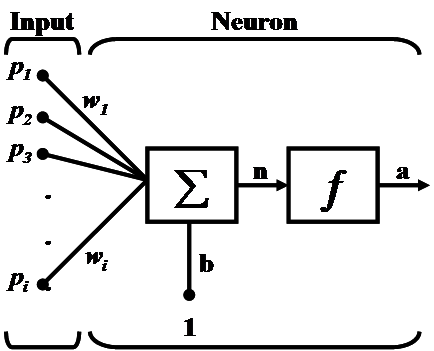
\includegraphics[width=.5\textwidth]{Figures/perceptron.png}
    \caption{Schematic representation of the perceptron extracted from~\cite{cortina2010analysis}.}
    \label{fig:perceptron}
\end{figure}



\begin{table}[h]
    \centering
\begin{tabular}{|c|c|}
\hline 
Activation function & Formula \tabularnewline
\hline 
Sigmoid & $f(x)= \frac{1}{1+ e^{-x}}$\tabularnewline
\hline 
Hyperbolic Tangent & $f(x)= \frac{1-e^{-2x}}{1+e^{-2x}}$\tabularnewline
\hline 
Rectified Linear units & $f(x)= max(x,0)$\tabularnewline
\hline 
\end{tabular}
    \caption{Commonly used activation functions in ANN}
    \label{tab:activation_func}
\end{table}


The problem of a perceptron is that it can not learn nonlinearly separable datasets. To solve this problem, we can add several perceptrons to form a layer and also introducing further layers. In this way, we have a multilayer feedforward neural network. In general, there are three types of layers in ANN namely input layer, hidden layer, and output layer. The goal of the input layer is to distribute incoming signals to the next layer and by definition, its units are not perceptron. However, the units in all layers after the input layer and output layer are perceptron since they communicate with the environment by sending or receiving messages to units in the layers to which they are connected. The output layer provides a link between the network and environment by submitting the processed information. In a classification problem, the number of units in the output layer is equal to the number of class labels~\cite{sharma2008high}. In training the network, its parameters ($w_i$) are adjusted so that the difference between the output units and the target values is minimized. There are several ways to train an ANN such as Resilient Backpropagation~\cite{riedmiller1993direct}, Scaled Conjugate Gradient~\cite{moller1993scaled} and Levenberg–Marquardt backpropagation~\cite{hagan1994training}. 






\chapter{Results}\label{chap:result}
In this section, the impact of the overlapping and non-overlapping sliding windows in HAR systems with Subject-dependent CV and Subject-independent CV for both datasets is evaluated. The experiments are categorized into global evaluation and activity-specific analysis. 


For each experiment, we report distributions of average F1-score values obtained across all validation folds. Each distribution contains 28 measures obtained for the different window sizes mentioned in Section~\ref{sec:experiment setup}. We selected this representation over 
summary statistics or confusion matrix as it provides a comprehensive and synthetic overview of classification performance over a range of window sizes, classifiers, and feature sets.
In all the figures of this section, “O” and “NO” stand for overlapping and non-overlapping windowing respectively. Non-overlapping windowing is represented in green, and overlapping windowing is in red.    
% We report distributions of  F1-score values across window sizes, we plot the distribution of the F1-scores, so as to  visually compare the classifiers performances in overlapping and non-overlapping sliding windows techniques. 
\section{Global evaluation}\label{global_evaluation}
In this set of experiments, we analyze the general impact of overlapping and non-overlapping windowing in HAR systems trough the average performance of models for different activities and window sizes. 
\subsubsection{Experiment 1: Subject-dependent CV} \label{sec:ex1}
In this experiment, we apply non-overlapping and overlapping windowing with subject-dependent CV and use it as a baseline
for further evaluations. 

We applied the ARP system as explained in Section~\ref{sec:experiment setup}, on the datasets described in Section~\ref{sec:dataset}. For each window size, we partitioned the dataset in non-overlapping and overlapping windows separately and extracted feature sets FS1, FS2, and FS3 in each window. We trained the classifiers on the resulting feature vectors, and measured their average F1-score over 10-fold CV.

\noindent\textbf{Dataset~1.} Figure~\ref{fig:exp1_ds1} shows the distribution of the F1-scores of the classifiers for different window sizes in overlapping and non-overlapping windows. The classifiers can be categorized in two groups: (1) KNN and DT, that have very different performance distributions for overlapping and non-overlapping windowing, and (2) NB and NCC, that show almost similar distributions for both techniques. Our findings show that, in general, using overlapping windowing improves the performance of all classifiers in all feature sets. Regarding the first group (KNN and DT), quantitatively, using the overlapping windowing technique improves the F1-score of the KNN and DT by about 10\%, 8\% and 8\% on average in FS1, FS2, and FS3 respectively. However, the improvement for the second group is about 1\%, on average, for all features sets, which is insignificant.

\noindent\textbf{Dataset~2.} The distribution of F1-scores for different window sizes and classifiers for overlapping and non-overlapping windowing is shown in Figure~\ref{fig:exp1_ds2}. Generally, the trends for Dataset 2 and Dataset 1 are similar. Overlapping windowing increases the F1-score and we observe the same two performance groups as before. The F1-score distributions of DT and KNN for overlapping and non-overlapping windowing are very different. Quantitatively, using overlapping sliding windows increases the performance of KNN and DT by about 9\%, 12\% and 13\% on average in FS1, FS2, and FS3 respectively. Regarding the NB and NCC, however, the increase is minor to negligible for all feature sets. 

These results show that using the overlapping windowing technique rather than the non-overlapping one in subject-dependent CV improves the performance of classifiers. This agreement between our results and the general argument of the effectiveness of overlapping windowing in HAR systems~\cite{janidarmian2017comprehensive,janidarmian2014automated}
reinforces our confidence in the correctness of our analysis method and its applicability to our next experiments.  



\subsubsection{Experiment 2: Subject-independent CV} \label{sec:ex2}
As explained in Section~\ref{sub:CVs},  subject-independent CV should be used to evaluate the performance of HAR systems. Thus, in this experiment, we compare the overlapping and non-overlapping windowing techniques when using subject-independent CV.  The only difference between this experiment and Experiment 1 is the use of subject-independent CV rather than subject-dependent CV.



\noindent\textbf{Dataset~1.} Figure~\ref{fig:exp2_ds1} shows our results. Similar to Experiment 1 for this dataset, we observed the same two performance groups among classifiers. Regarding the first group (KNN and DT), however, overlapping windows do not lead to any improvement of the F1-score compared to non-overlapping windows. Overlapping windows even slightly decrease the F1-scores of DT and KNN in all feature sets, on average by 2\% (FS1), 4\% (FS2) and 1\% (FS3). To further illustrate this result, Table~\ref{tab:ds-fs3-f1score} shows the F1-score of DT and KNN for several window sizes in overlapping and nonoverlapping windowing techniques for FS3: the performance of overlapping and non-overlapping windows is very similar.  For NB and NCC the F1-scores obtained with both techniques are similar for all feature sets.

\noindent\textbf{Dataset~2.} Figure~\ref{fig:exp2_ds2} shows the results of Experiment~2 for Dataset~2. Once again, the F1-scores obtained for overlapping and nonoverlapping windows are very similar.
This time, with DT and KNN, overlapping windowing improves the F1-scores slightly compared to non-overlapping windowing, on average by 2\% (FS1), 1\% (FS2) and 1\% (FS3). The comparison between the performance of KNN and DT for several window size is shown in Table~\ref{tab:ds-fs3-f1score}. For NB and NCC the F1-scores obtained with both techniques are similar for all feature sets.

\begin{table}[]
    \centering
% Preview source code for paragraph 0
\begin{tabular}{|>{}c|>{}c|>{}c|>{}c|>{}c|}
\hline 
Dataset & window size (sec) & Classifier & F1-score - O (\%) & F1-score - NO (\%)\tabularnewline
\hline 
\multirow{8}{*}{1} & \multirow{2}{*}{1} & DT & 86.42 & 86.0\tabularnewline
\cline{3-5} \cline{4-5} \cline{5-5} 
 &  & KNN & 89.04 & 88.78\tabularnewline
\cline{2-5} \cline{3-5} \cline{4-5} \cline{5-5} 
 & \multirow{2}{*}{4} & DT & 81.97 & 83.38\tabularnewline
\cline{3-5} \cline{4-5} \cline{5-5} 
 &  & KNN & 82.05 & 82.18\tabularnewline
\cline{2-5} \cline{3-5} \cline{4-5} \cline{5-5} 
 & \multirow{2}{*}{6} & DT & 80.1 & 80.83\tabularnewline
\cline{3-5} \cline{4-5} \cline{5-5} 
 &  & KNN & 79.08 & 79.30\tabularnewline
\cline{2-5} \cline{3-5} \cline{4-5} \cline{5-5} 
 & \multirow{2}{*}{7} & DT & 80.61 & 80.62\tabularnewline
\cline{3-5} \cline{4-5} \cline{5-5} 
 &  & KNN & 77.74 & 78.68\tabularnewline
\hline 
\multirow{8}{*}{2} & \multirow{2}{*}{1} & DT & 69.26 & 67.38\tabularnewline
\cline{3-5} \cline{4-5} \cline{5-5} 
 &  & KNN & 63.61 & 63.94\tabularnewline
\cline{2-5} \cline{3-5} \cline{4-5} \cline{5-5} 
 & \multirow{2}{*}{4} & DT & 74.37 & 73.06\tabularnewline
\cline{3-5} \cline{4-5} \cline{5-5} 
 &  & KNN & 65.52 & 67.01\tabularnewline
\cline{2-5} \cline{3-5} \cline{4-5} \cline{5-5} 
 & \multirow{2}{*}{6} & DT & 75.28 & 73.12\tabularnewline
\cline{3-5} \cline{4-5} \cline{5-5} 
 &  & KNN & 66.0 & 67.8\tabularnewline
\cline{2-5} \cline{3-5} \cline{4-5} \cline{5-5} 
 & \multirow{2}{*}{7} & DT & 75.46 & 73.06\tabularnewline
\cline{3-5} \cline{4-5} \cline{5-5} 
 &  & KNN & 66.0 & 67.93\tabularnewline
\hline 
\end{tabular}


    \caption{F1-scores of DT and KNN for several window sizes in overlapping (O) and nonoverlapping (NO) windowing -- Subject-independent CV -- FS3.}
    \label{tab:ds-fs3-f1score}
\end{table}

In general, compared to Experiment~1 for both datasets, the performance of all classifiers in all feature sets decreased which may be due to the overestimation of subject-dependent CV. In other words, subject-independent CV removes the performance improvement resulting from using overlapping windows in Experiment~1 which seems to be resulted from the overestimation of subject-dependent CV. This experiment shows that the performance advantage of overlapping windows in the literature seems to be due to the use of subject-dependent CV and in case of using subject-independent CV, this method does not offer any benefit to the performance of HAR systems. Hence, we can reach to the same recognition performance by using non-overlapping windows. Considering the resource-intensity of overlapping windowing compared to non-overlapping one,  this is an important conclusion since through that we can save a lot of resources (energy, time, etc) which is a desirable feature in HAR~\cite{lara2012survey}.   



\begin{figure}[htp]
  \centering
  \subfigure[FS1]{\label{fig:ds1-FS1-exp1}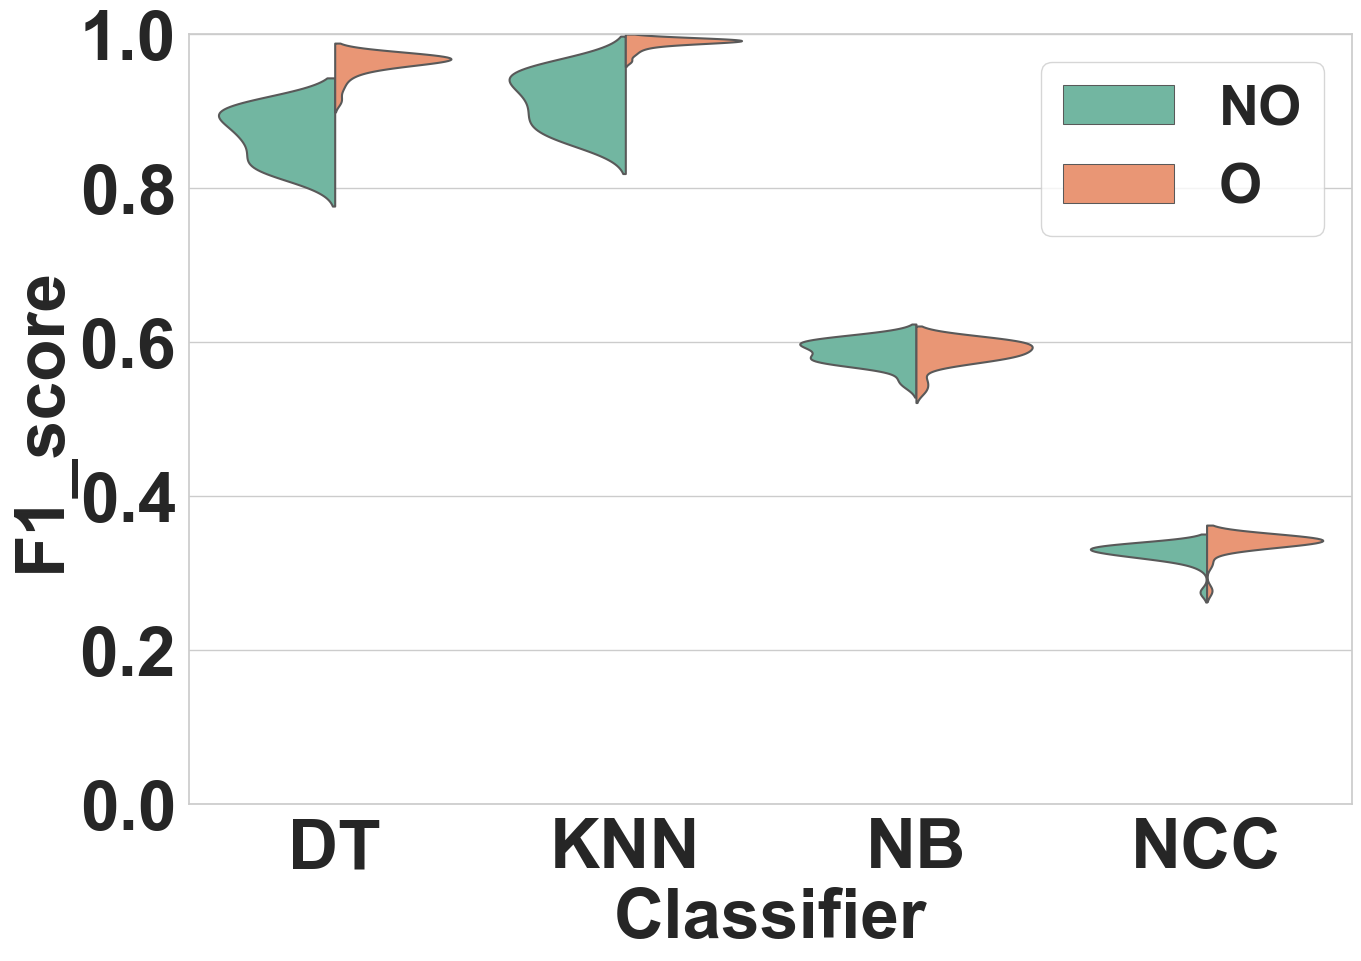
\includegraphics[scale=0.14]{Figures/Dataset1_iid_FS1.png}}\quad
  \subfigure[FS2]{\label{fig:ds1-FS2-exp1}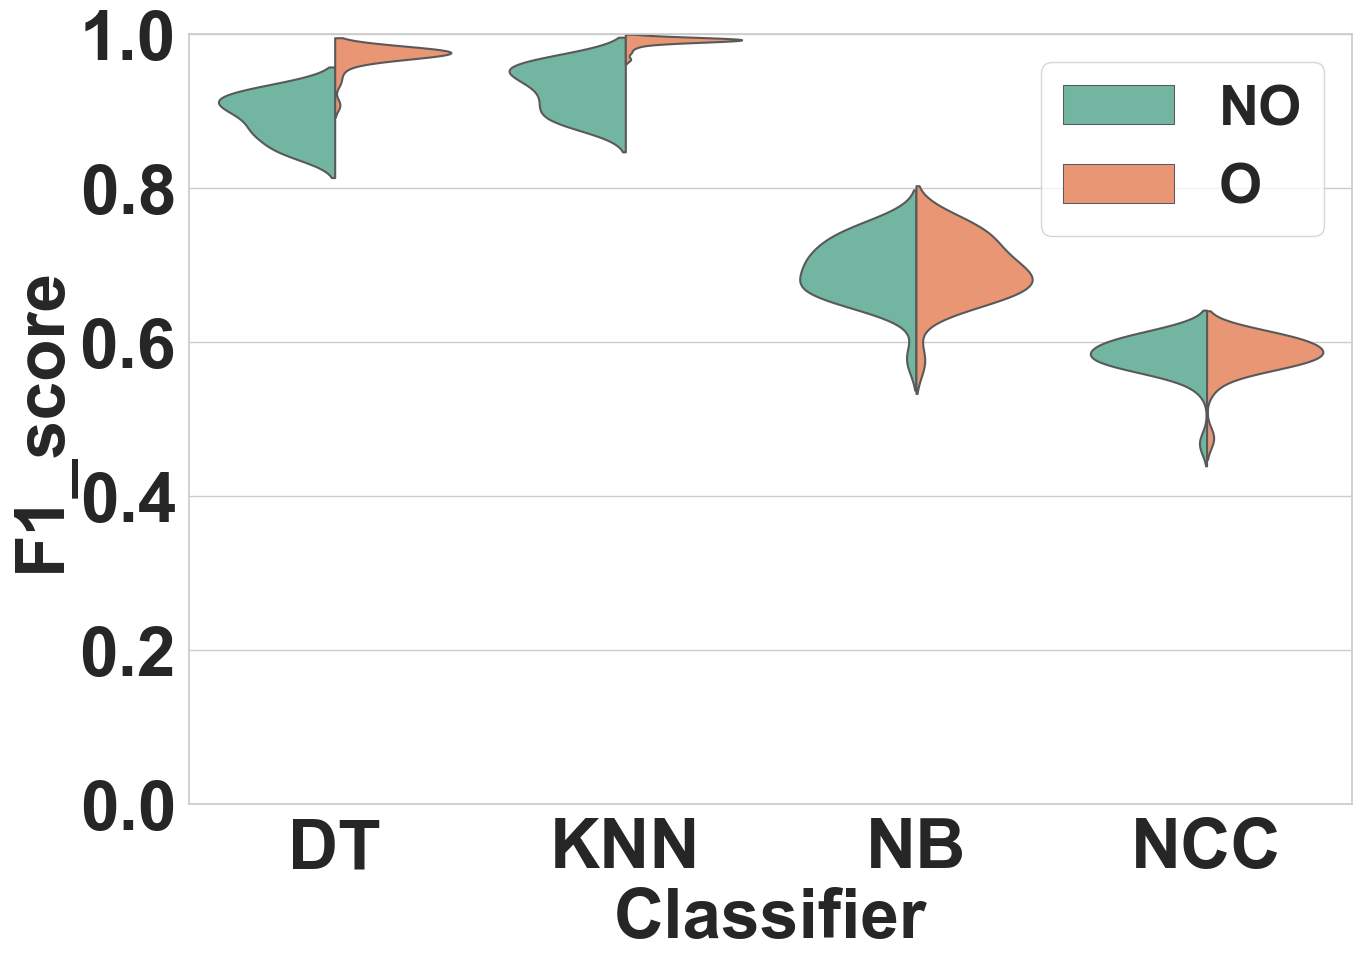
\includegraphics[scale=0.14]{Figures/Dataset1_iid_FS2.png}}
  \subfigure[FS3]{\label{fig:ds1-FS3-exp1}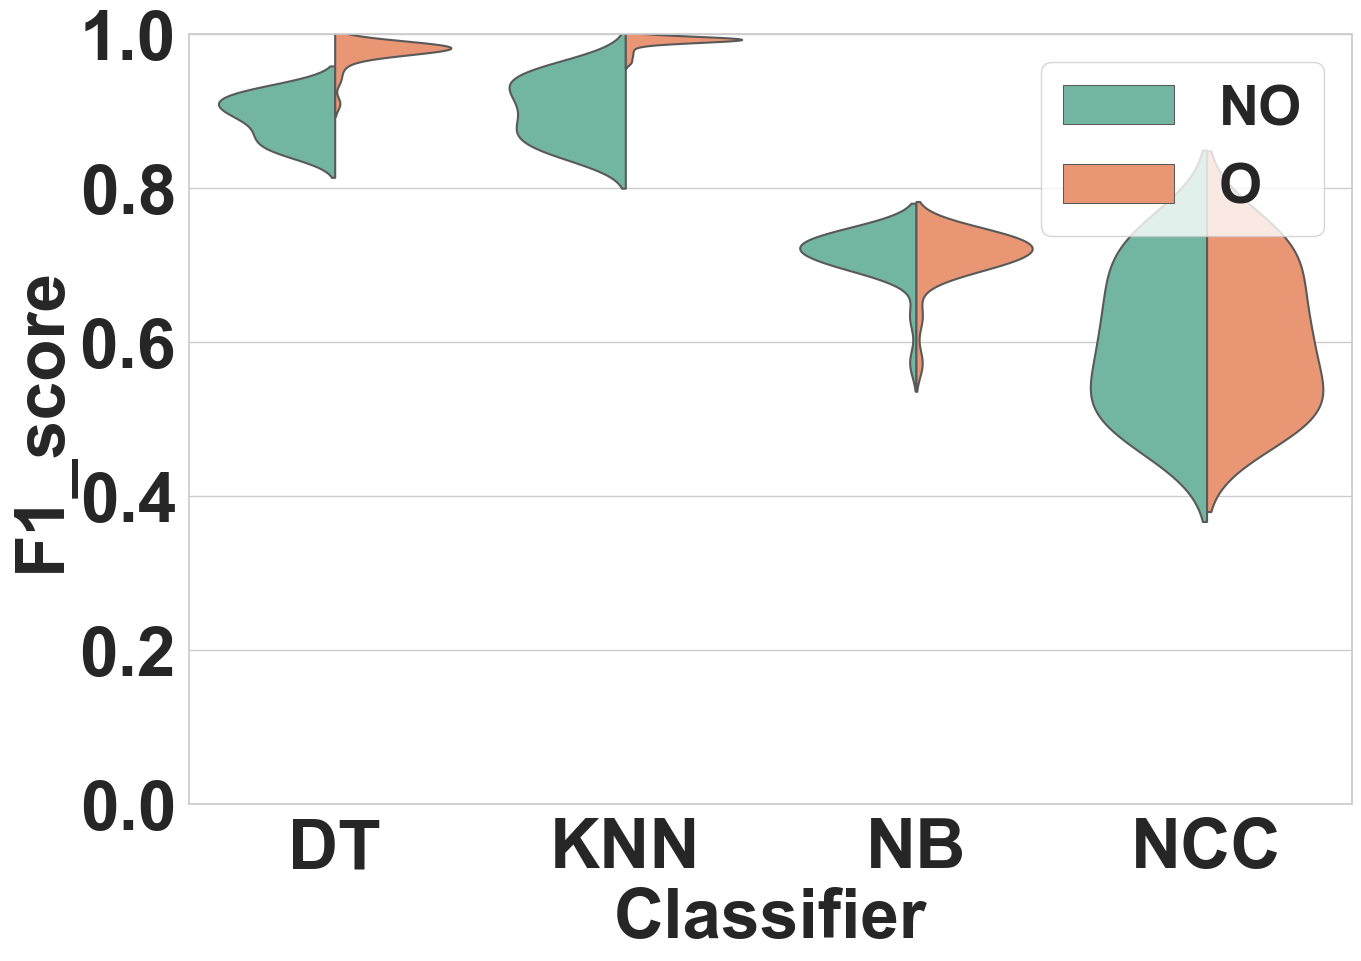
\includegraphics[scale=0.14]{Figures/Dataset1_iid_FS3.png}}
   
   \caption{Experiment 1 -- Subject-dependent CV -- Dataset 1.}
    \label{fig:exp1_ds1}
    
\end{figure}

\begin{figure}[htp]
  \centering
  \subfigure[FS1]{\label{fig:ds2-FS1-exp1}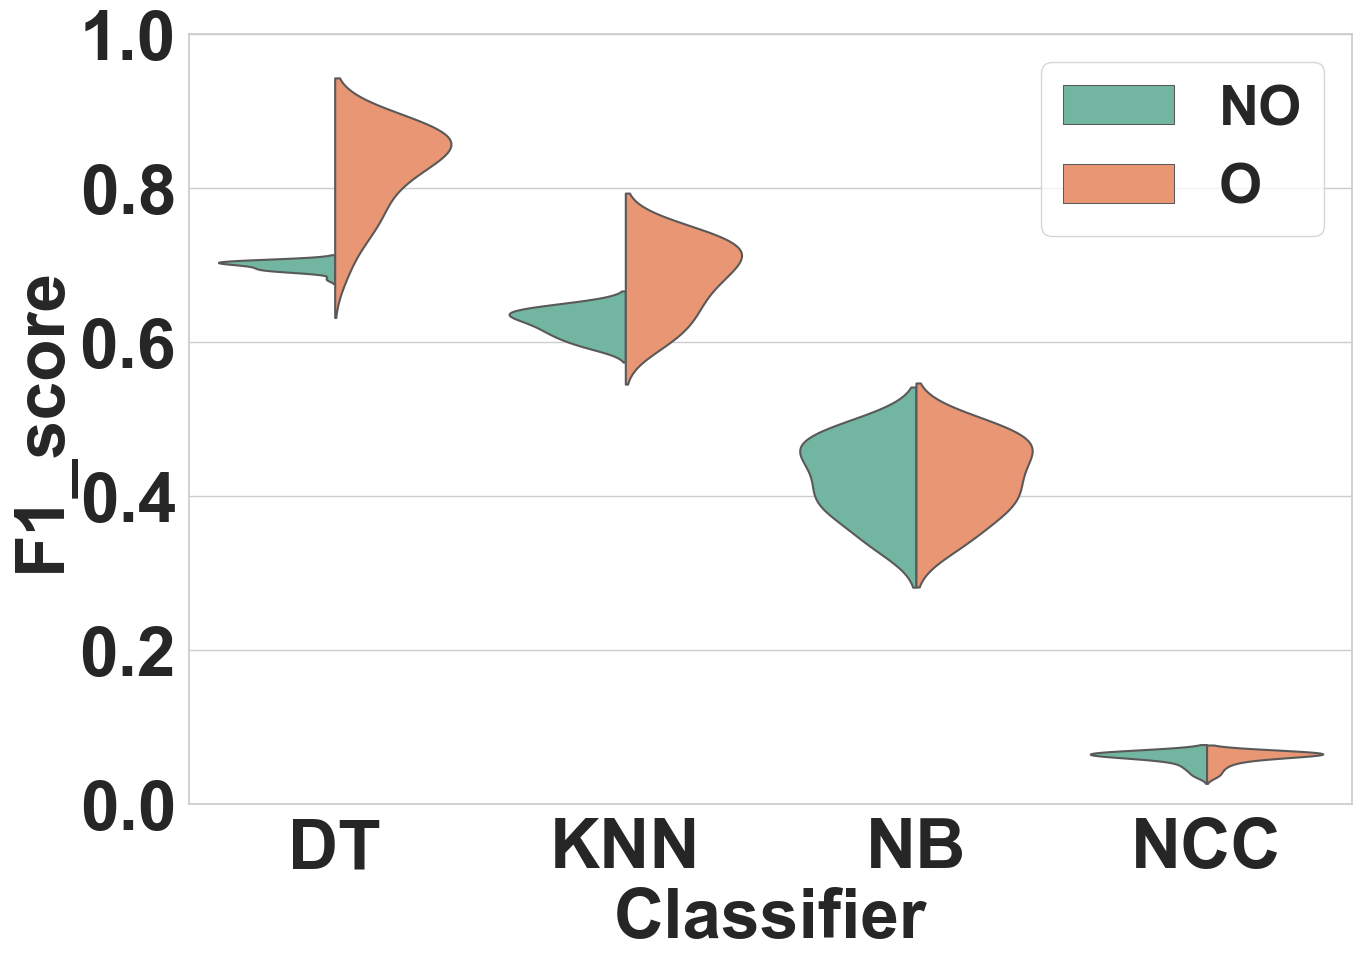
\includegraphics[scale=0.14]{Figures/Dataset2_iid_FS1.png}}\quad
  \subfigure[FS2]{\label{fig:ds2-FS2-exp1}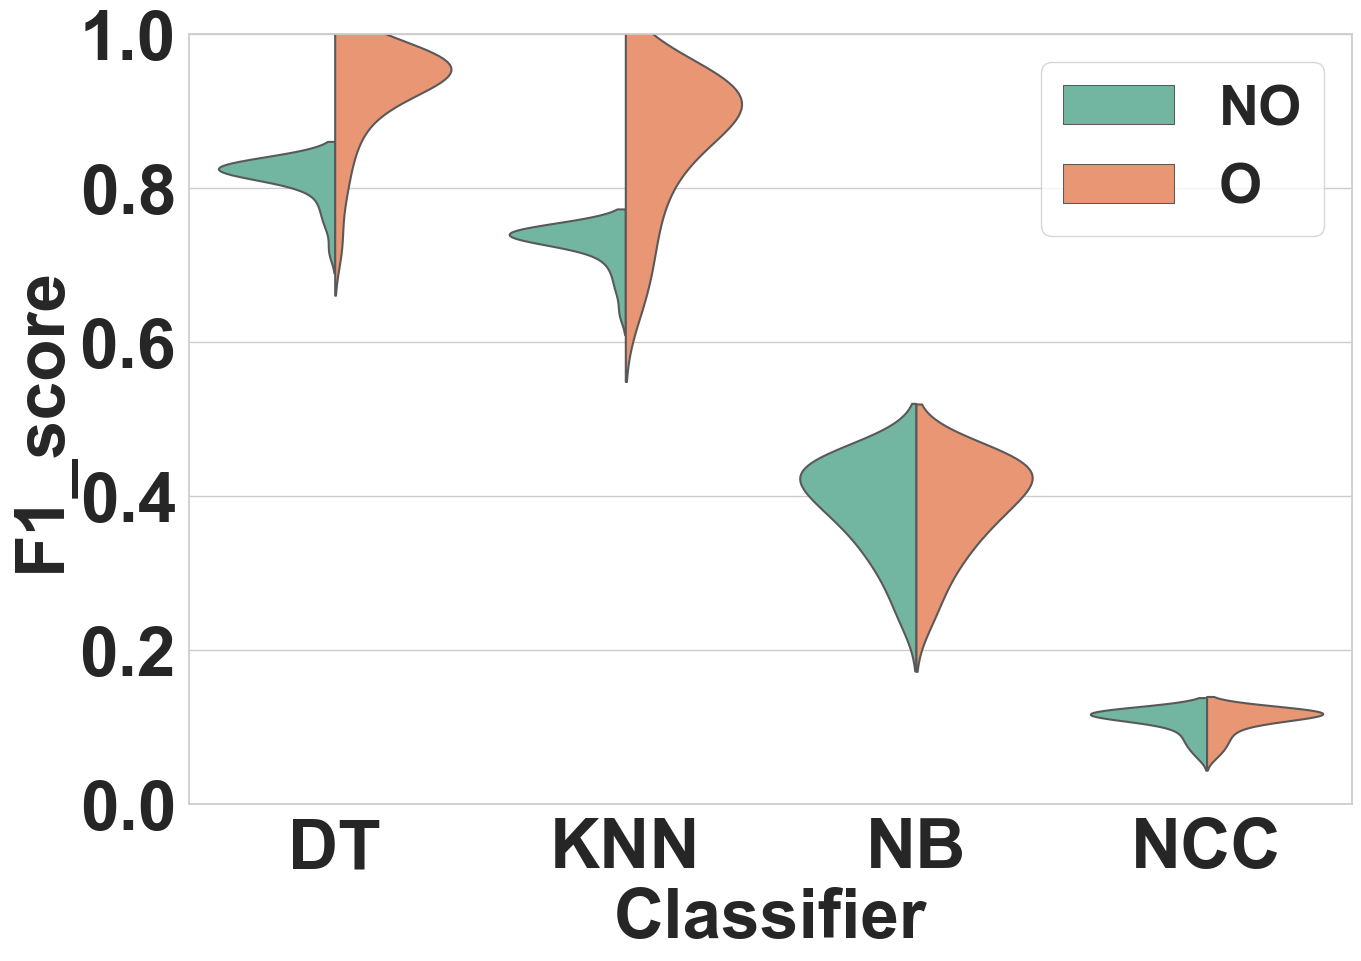
\includegraphics[scale=0.14]{Figures/Dataset2_iid_FS2.png}}
  \subfigure[FS3]{\label{fig:ds2-FS3-exp1}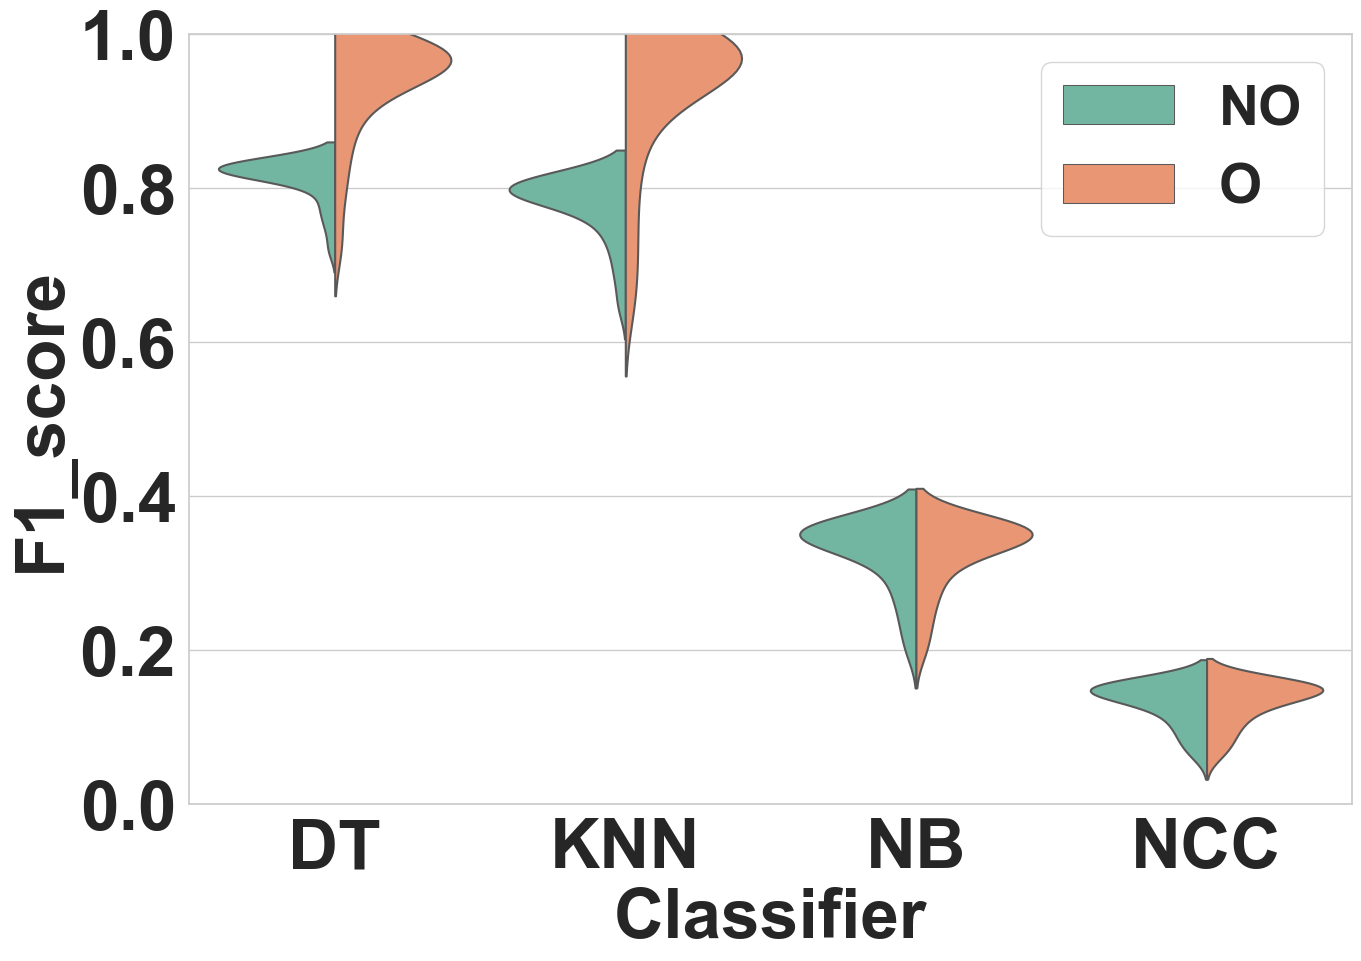
\includegraphics[scale=0.14]{Figures/Dataset2_iid_FS3.png}}
   
   \caption{Experiment 1 -- Subject-dependent CV -- Dataset 2. }
    \label{fig:exp1_ds2}
    
\end{figure}

\begin{figure}[htp]
  \centering
  \subfigure[FS1]{\label{fig:ds1-FS1-exp2}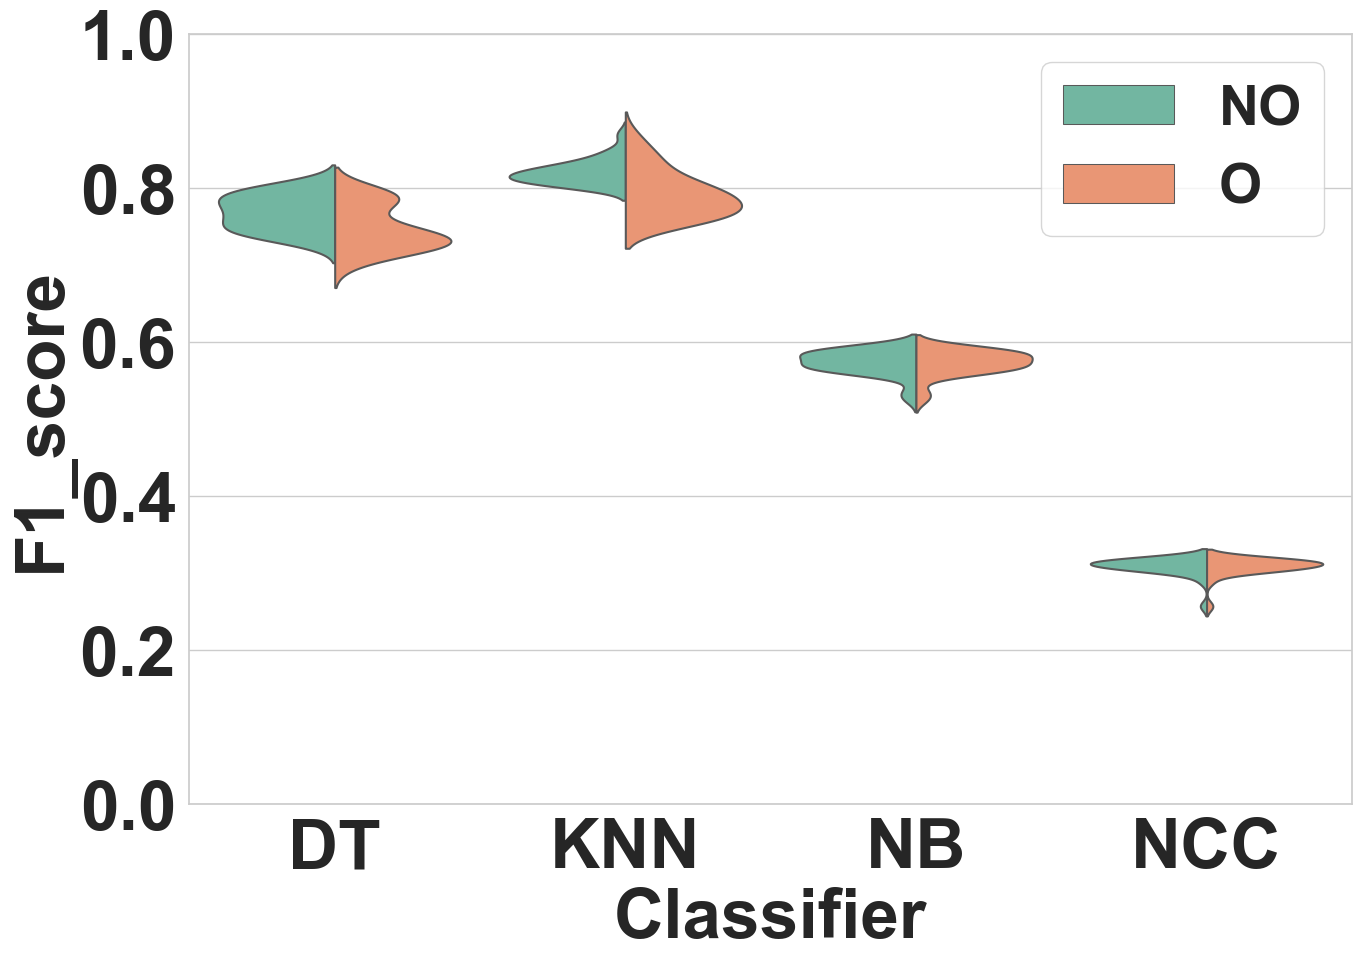
\includegraphics[scale=0.14]{Figures/Dataset1_sbj_FS1.png}}\quad
  \subfigure[FS2]{\label{fig:ds1-FS2-exp2}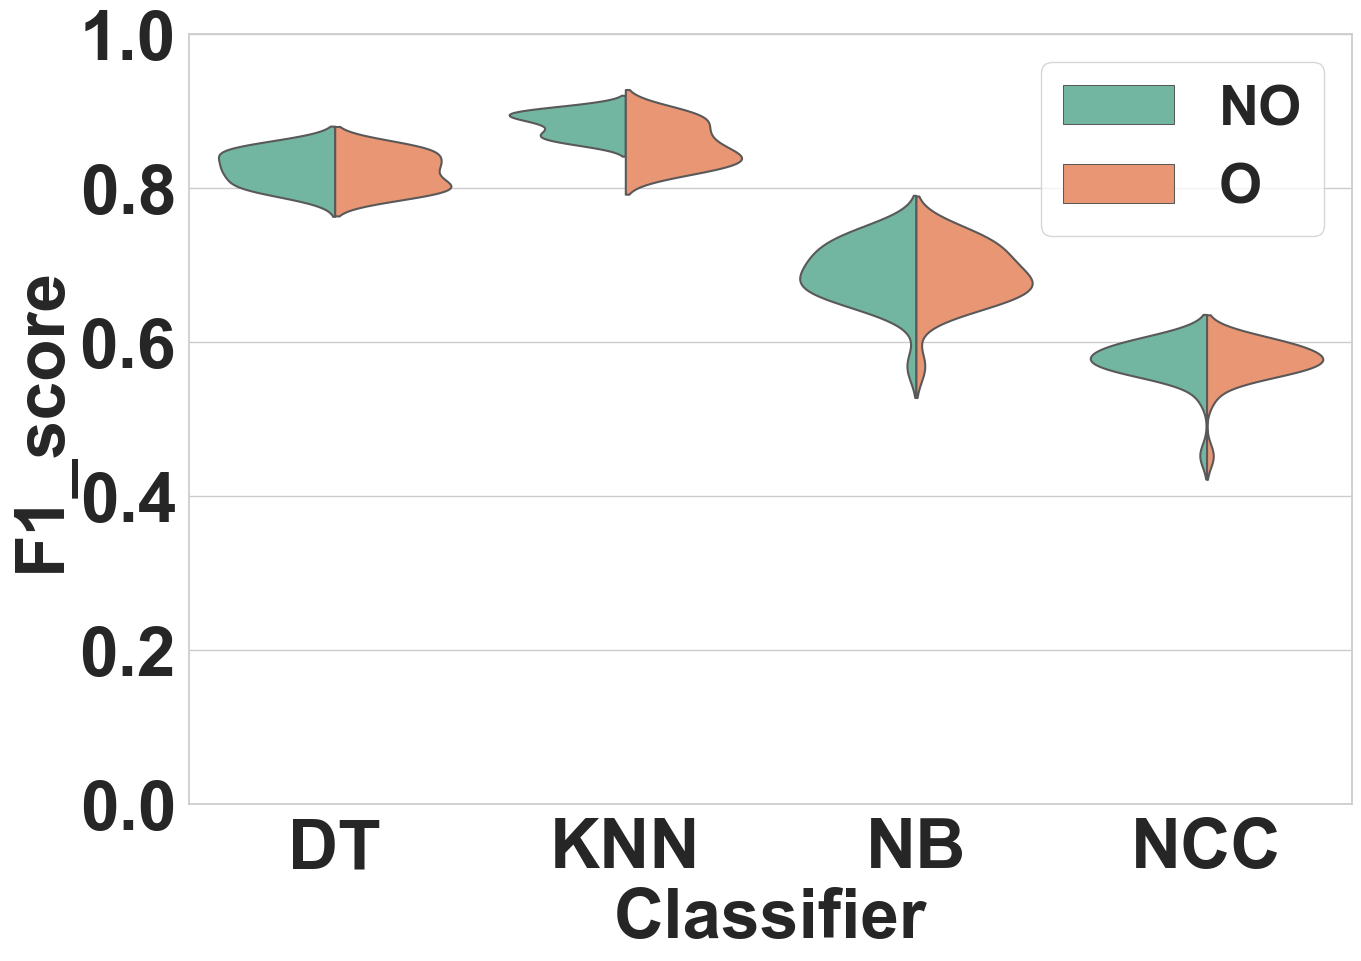
\includegraphics[scale=0.14]{Figures/Dataset1_sbj_FS2.png}}
  \subfigure[FS3]{\label{fig:ds1-FS3-exp2}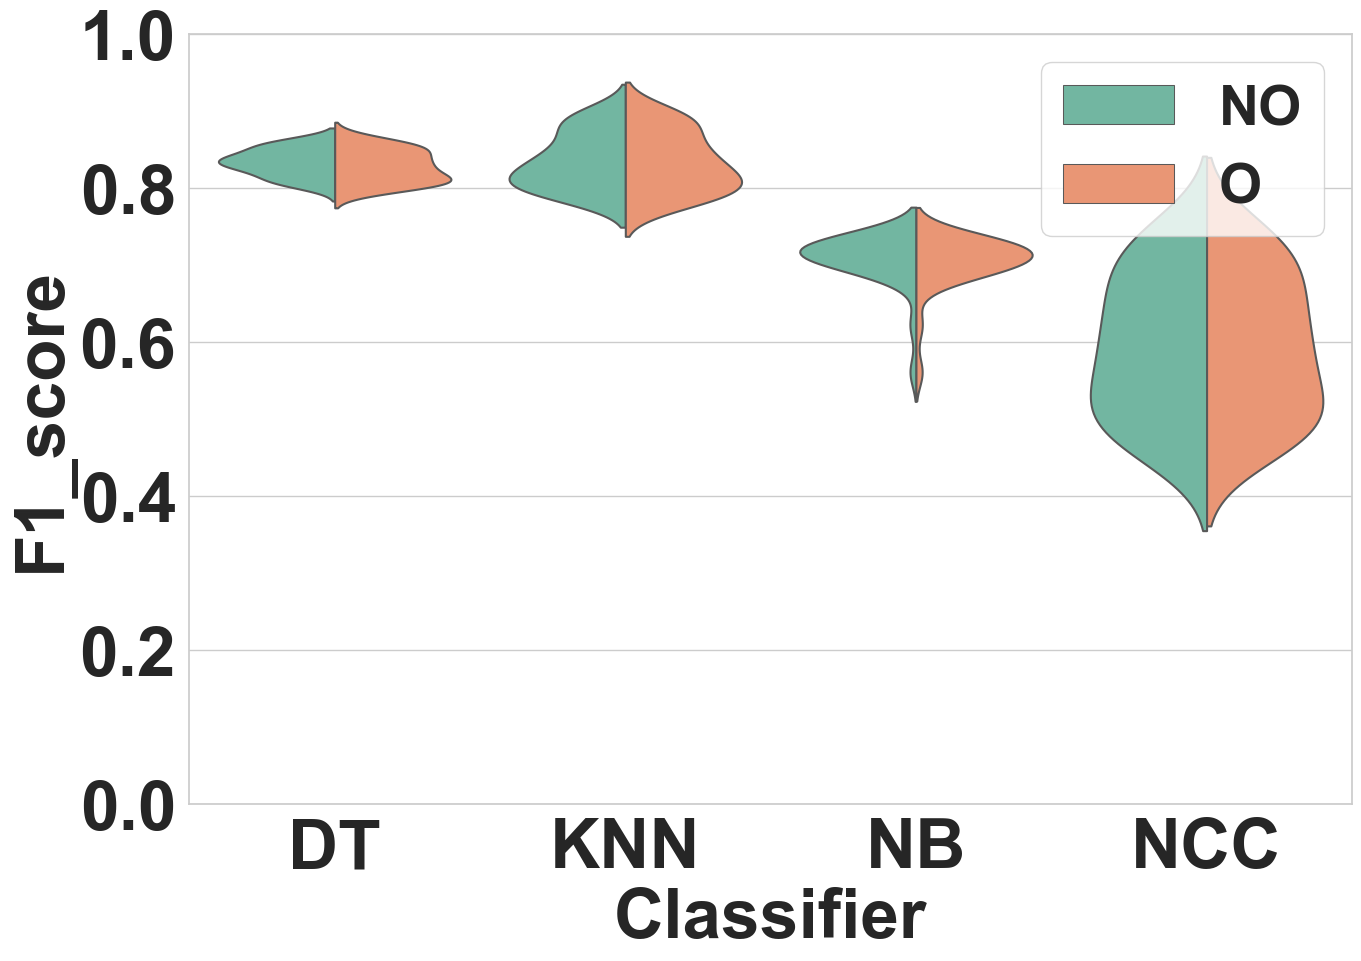
\includegraphics[scale=0.14]{Figures/Dataset1_sbj_FS3.png}}
   
   \caption{Experiment 2 -- Subject-independent CV -- Dataset 1.}
    \label{fig:exp2_ds1}
    
\end{figure}

\begin{figure}[htp]
  \centering
  \subfigure[FS1]{\label{fig:ds2-FS1-exp2}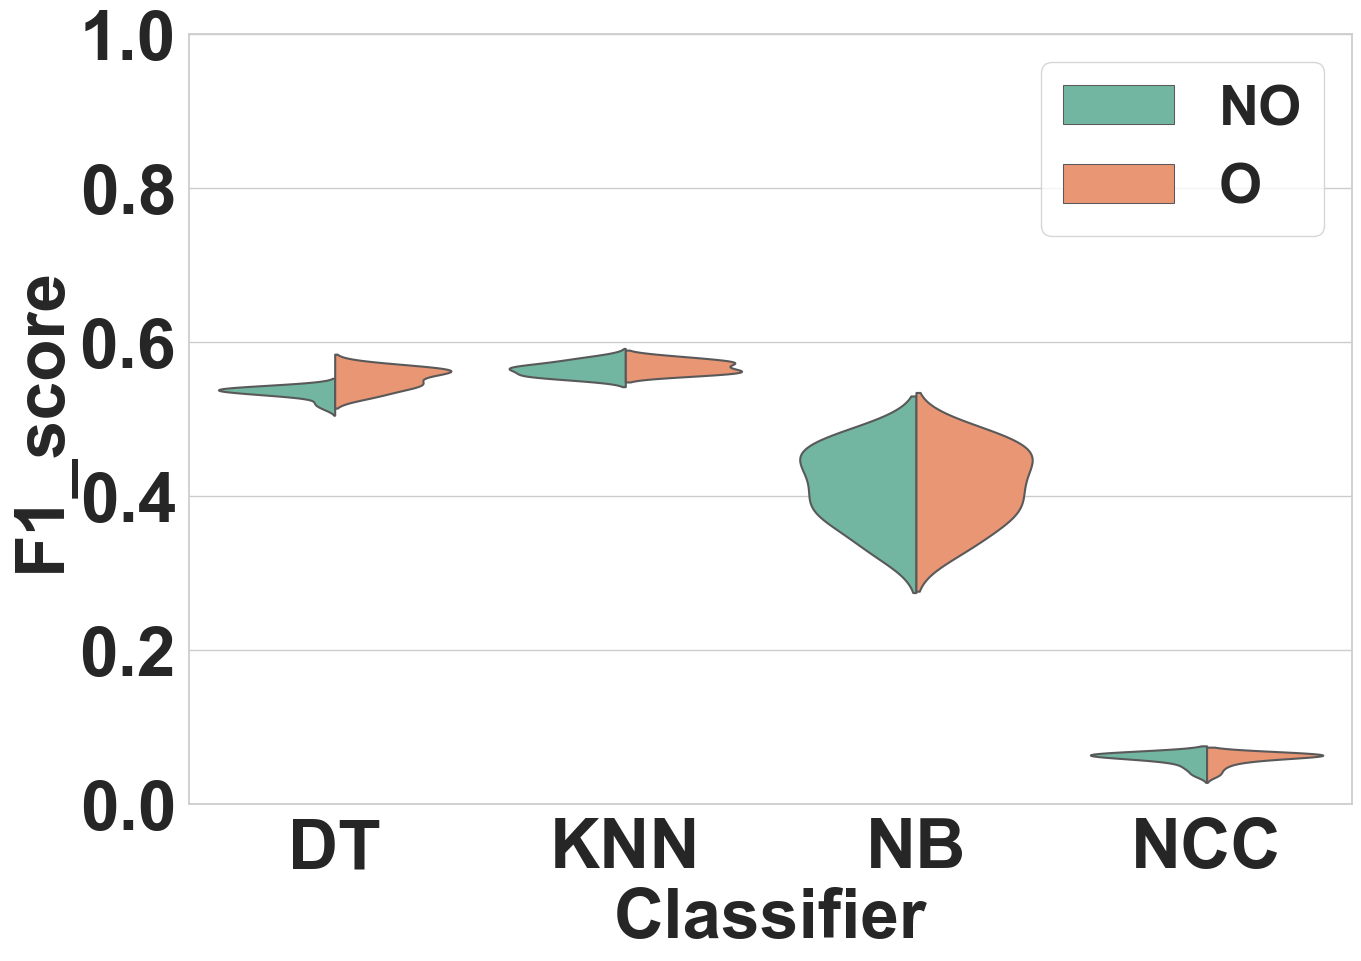
\includegraphics[scale=0.14]{Figures/Dataset2_sbj_FS1.png}}\quad
  \subfigure[FS2]{\label{fig:ds2-FS2-exp2}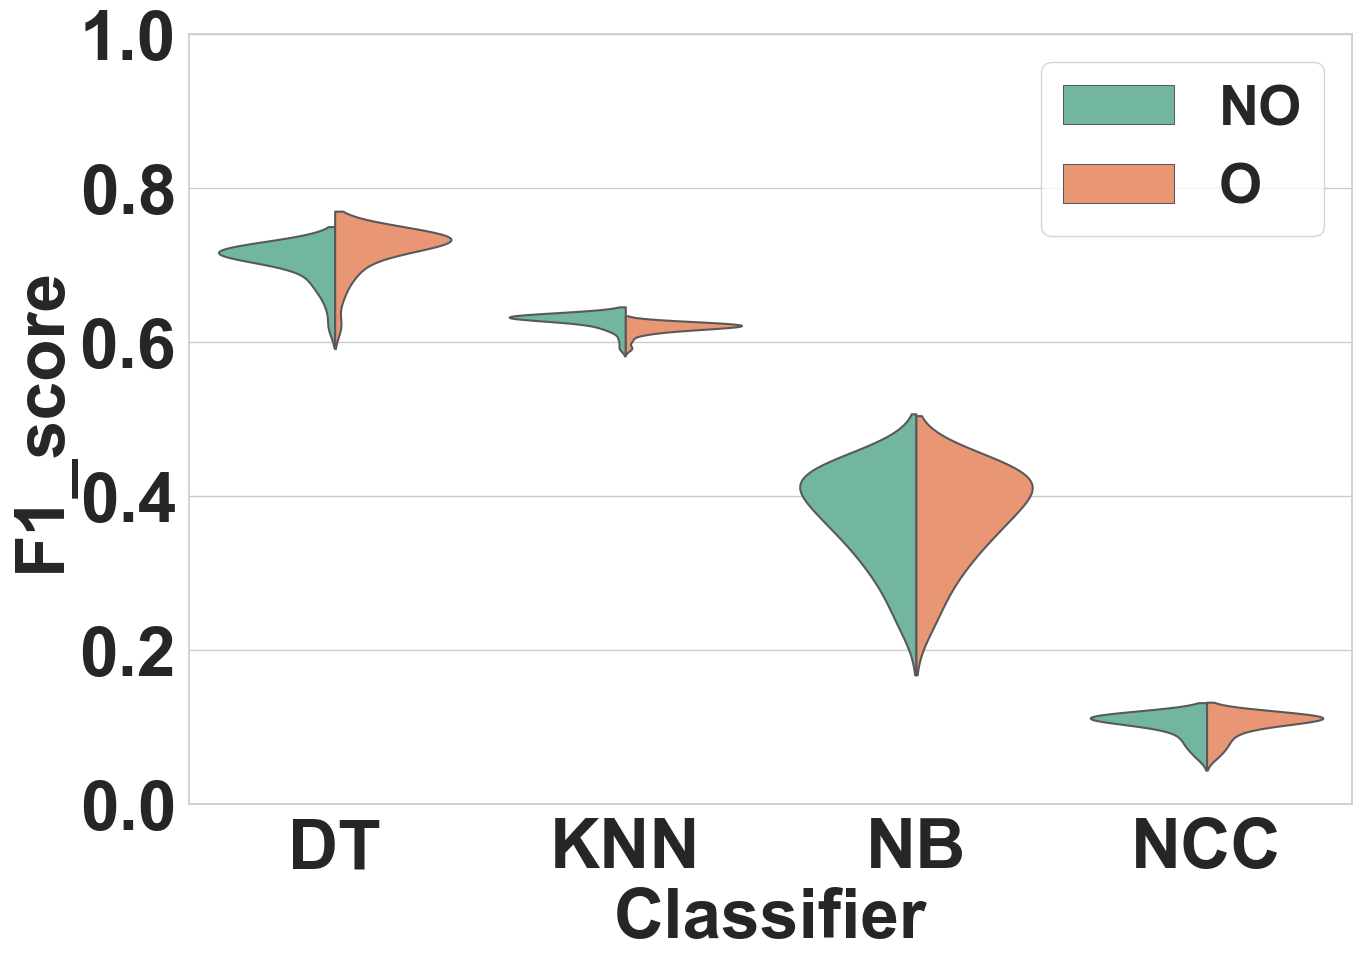
\includegraphics[scale=0.14]{Figures/Dataset2_sbj_FS2.png}}
  \subfigure[FS3]{\label{fig:ds2-FS3-exp2}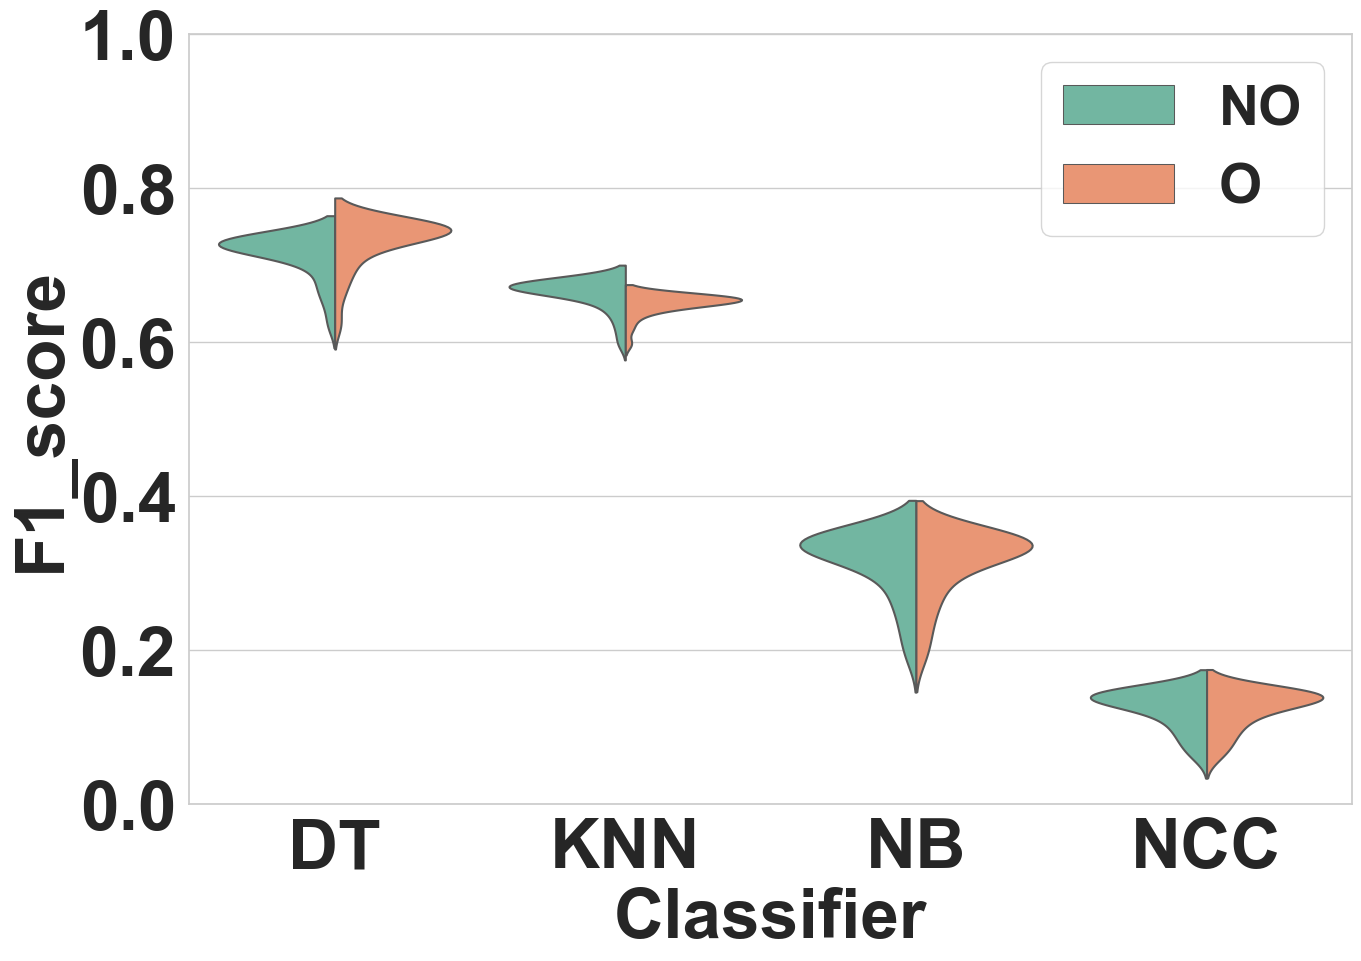
\includegraphics[scale=0.14]{Figures/Dataset2_sbj_FS3.png}}
   
   \caption{Experiment 2 -- Subject-independent CV -- Dataset 2.}
    \label{fig:exp2_ds2}
    
\end{figure}

\subsubsection{Experiment 3: Subject-independent CV and new hyperparameters } \label{sec:ex3}
One may claim that the results of Experiment~2 
are due to the specific set of hyperparameters used in the classifiers. Thus, to investigate that, we reproduced Experiment~2 with a new set of hyperparameters for the KNN and DT classifiers.

We selected new hyperparameter values such that (1) overfitting or underfitting does not occur, and (2) the new values are as different as possible from those in the previous experiments. Table~\ref{tab:hparams} compares the selected values for hyperparameters of DT and KNN in Experiment~1 and Experiment~2. 

\begin{table}[]
    \centering
\begin{tabular}{|>{}c|>{}c|>{}c|>{}c|}
\hline 
\multirow{1}{*}{Classifier} & Hyperparameter & Experiment~2 & Experiment~3\tabularnewline
\hline 
KNN & K (n\_neighbors) & 3 & 6\tabularnewline
\hline 
\multirow{3}{*}{DT} & Criterion & 'gini' & 'entropy'\tabularnewline
\cline{2-4} \cline{3-4} \cline{4-4} 
 & max\_depth & None & 20\tabularnewline
\cline{2-4} \cline{3-4} \cline{4-4} 
 & max\_features & 1 & 0.7\tabularnewline
\hline 
\end{tabular}
    \caption{The hyperparameters values for KNN and DT in Experiment~1 and Experiment~2. When max\_depth is set to None, the decision tree is expanded until all leaves are pure~\cite{pedregosa2011scikit}.}
    \label{tab:hparams}
\end{table}

\noindent\textbf{Dataset~1.} Results are shown in Figure~\ref{fig:exp3_ds1}. As in the previous experiments, the F1-scores obtained with overlapping and with non-overlapping windows are comparable. For DT, using overlapping windows decreases the performance in all feature sets, by about 1\%. As for KNN, using overlapping windowing reduces the F1-score by about 4\% in FS1 and FS2, and increases it by 1\% in FS3.   

\noindent\textbf{Dataset~2.} Figure~\ref{fig:exp3_ds2} shows our results for this dataset. The trend is similar to the previous experirments, i.e., F1-scores obtained with overlapping and with non-overlapping windowing are very similar. Qualitatively, such differences for both classifiers remain lower than 1\% in all feature sets.  

In conclusion, overlapping windowing does not provide any performance improvement compared to non-overlapping windowing with our new set of hyperparameters, which confirms the findings of Experiment 2.

% exp3 figures
\begin{figure}[htp]
  \centering
  \subfigure[FS1]{\label{fig:ds1-FS1-exp3}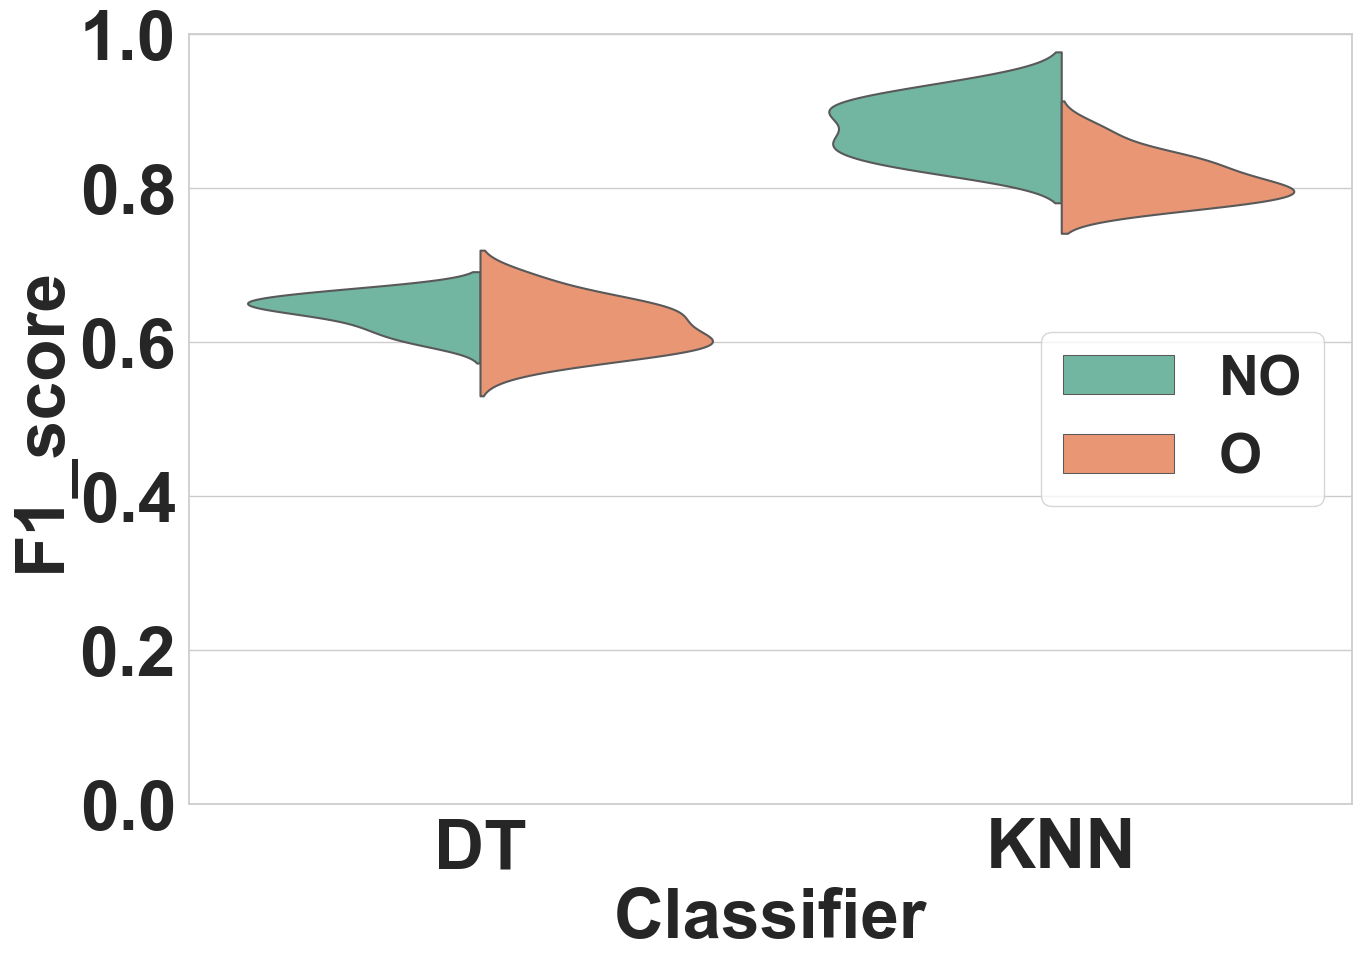
\includegraphics[scale=0.14]{Figures/Dataset1_sbj_FS1_new_hparams.png}}\quad
  \subfigure[FS2]{\label{fig:ds1-FS2-exp3}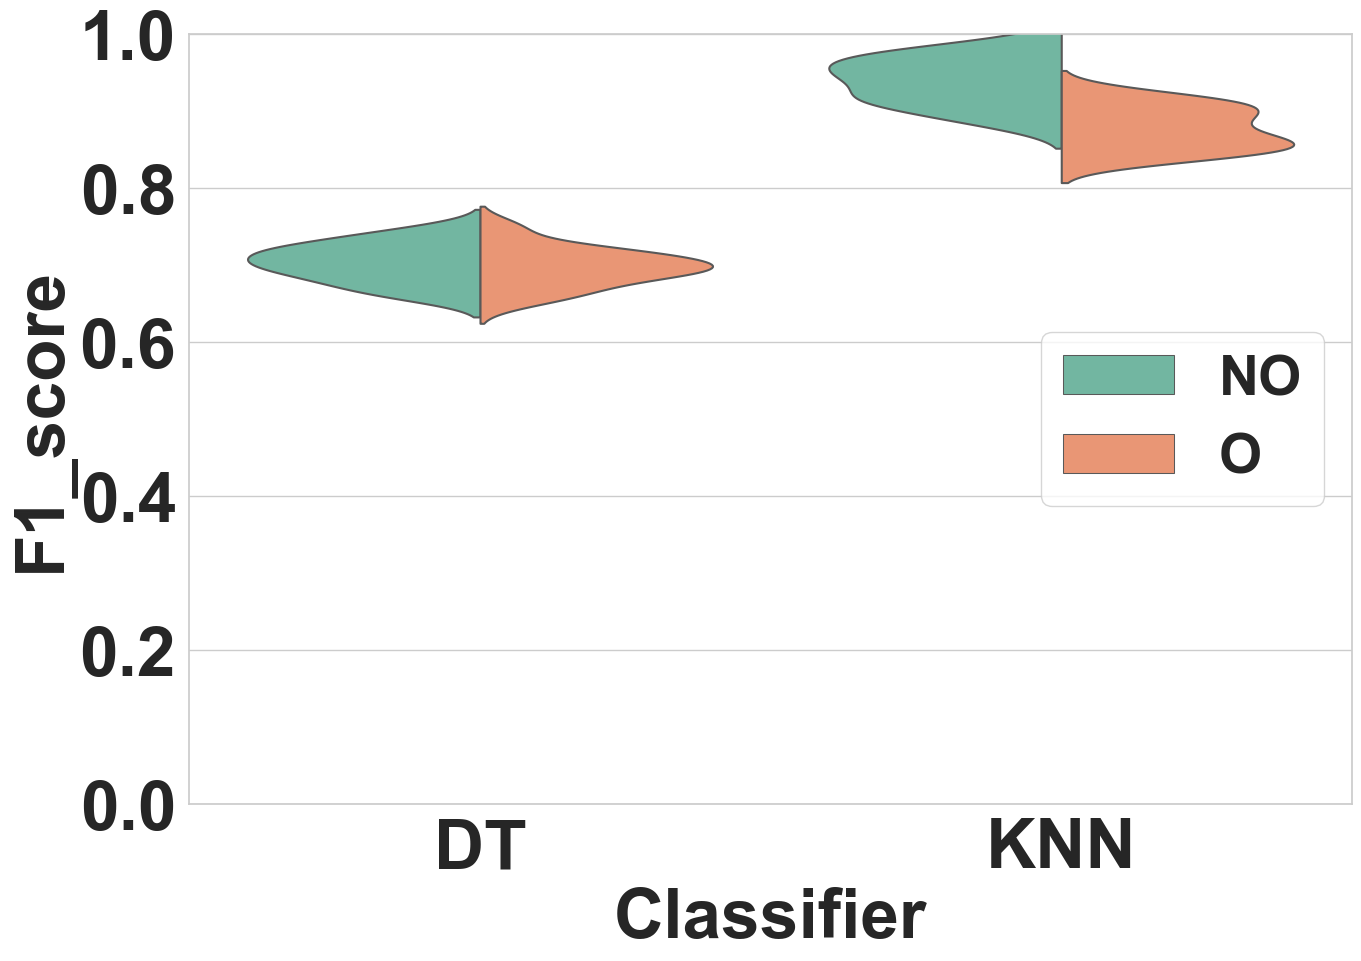
\includegraphics[scale=0.14]{Figures/Dataset1_sbj_FS2_new_hparams.png}}
  \subfigure[FS3]{\label{fig:ds1-FS3-exp3}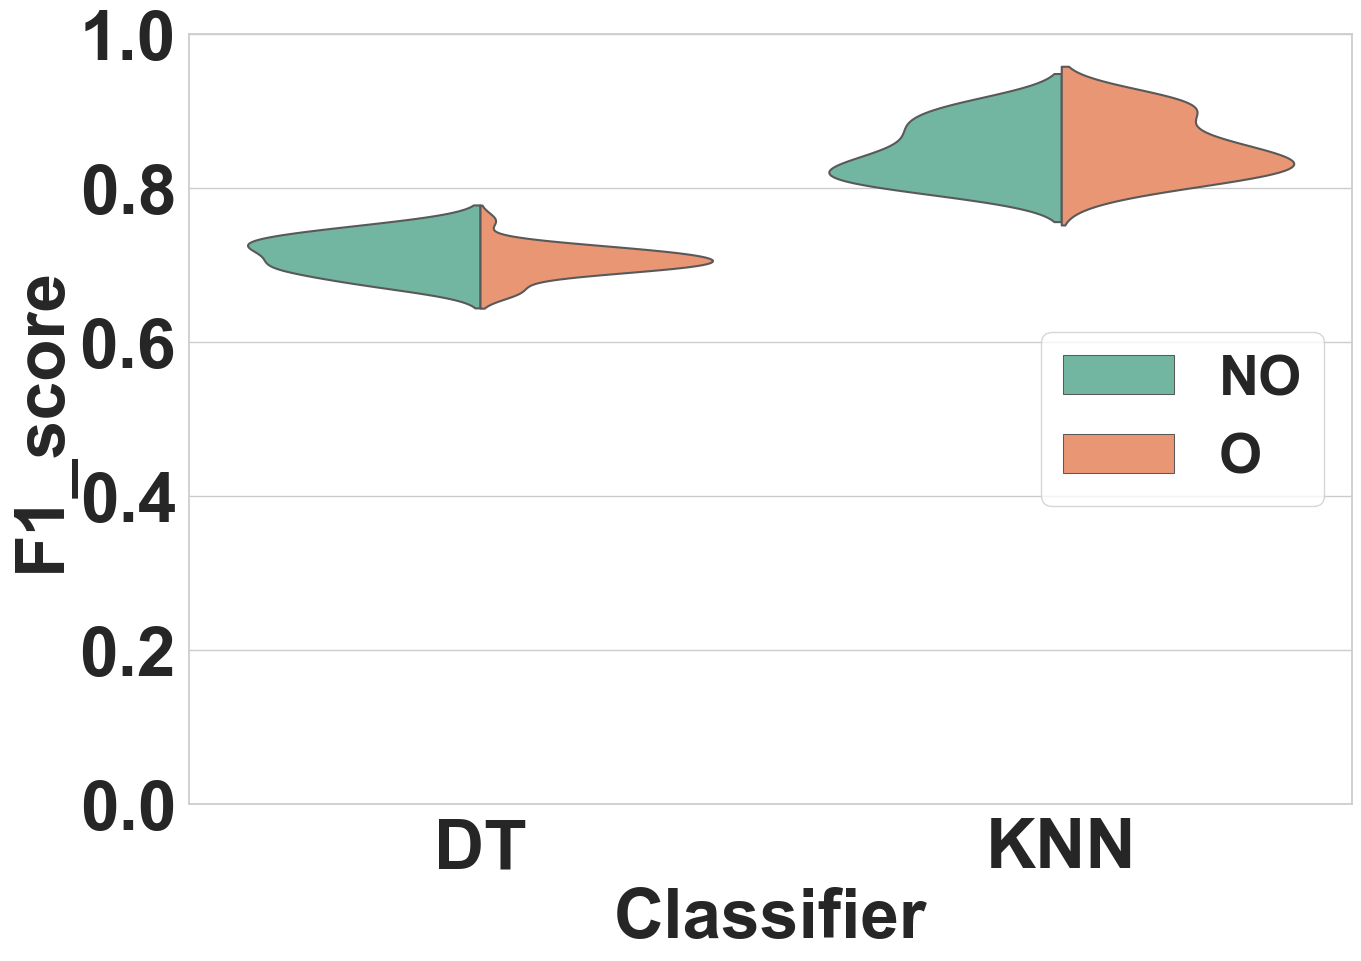
\includegraphics[scale=0.14]{Figures/Dataset1_sbj_FS3_new_hparams.png}}
   
   \caption{Experiment 3 -- Subject-independent CV -- Dataset 1.}
    \label{fig:exp3_ds1}
    
\end{figure}

\begin{figure}[htp]
  \centering
  \subfigure[FS1]{\label{fig:ds2-FS1-exp3}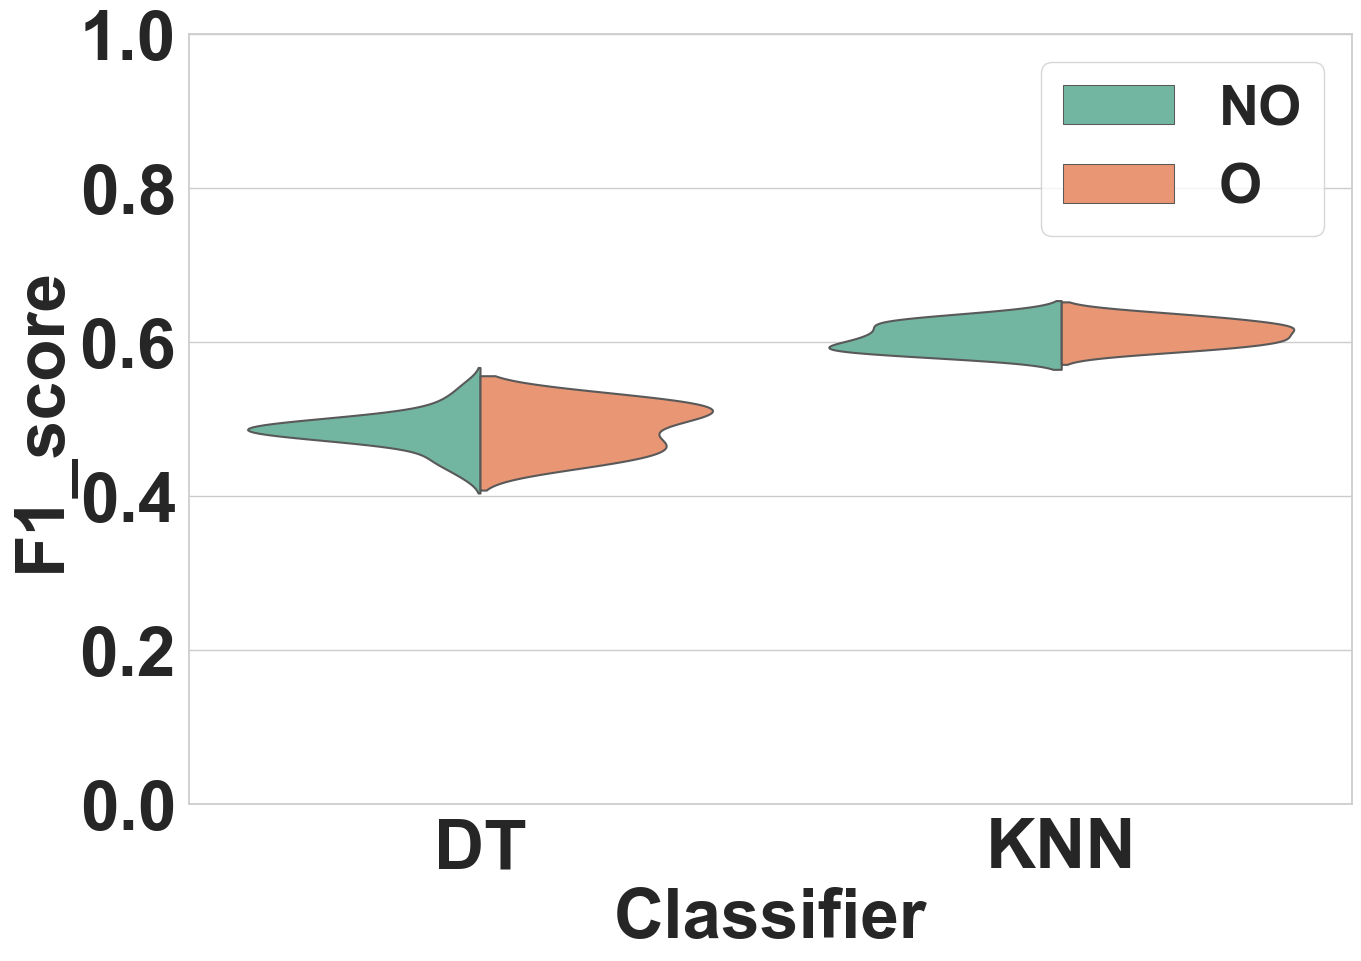
\includegraphics[scale=0.14]{Figures/Dataset2_sbj_FS1_new_hparams.png}}\quad
  \subfigure[FS2]{\label{fig:ds2-FS2-exp3}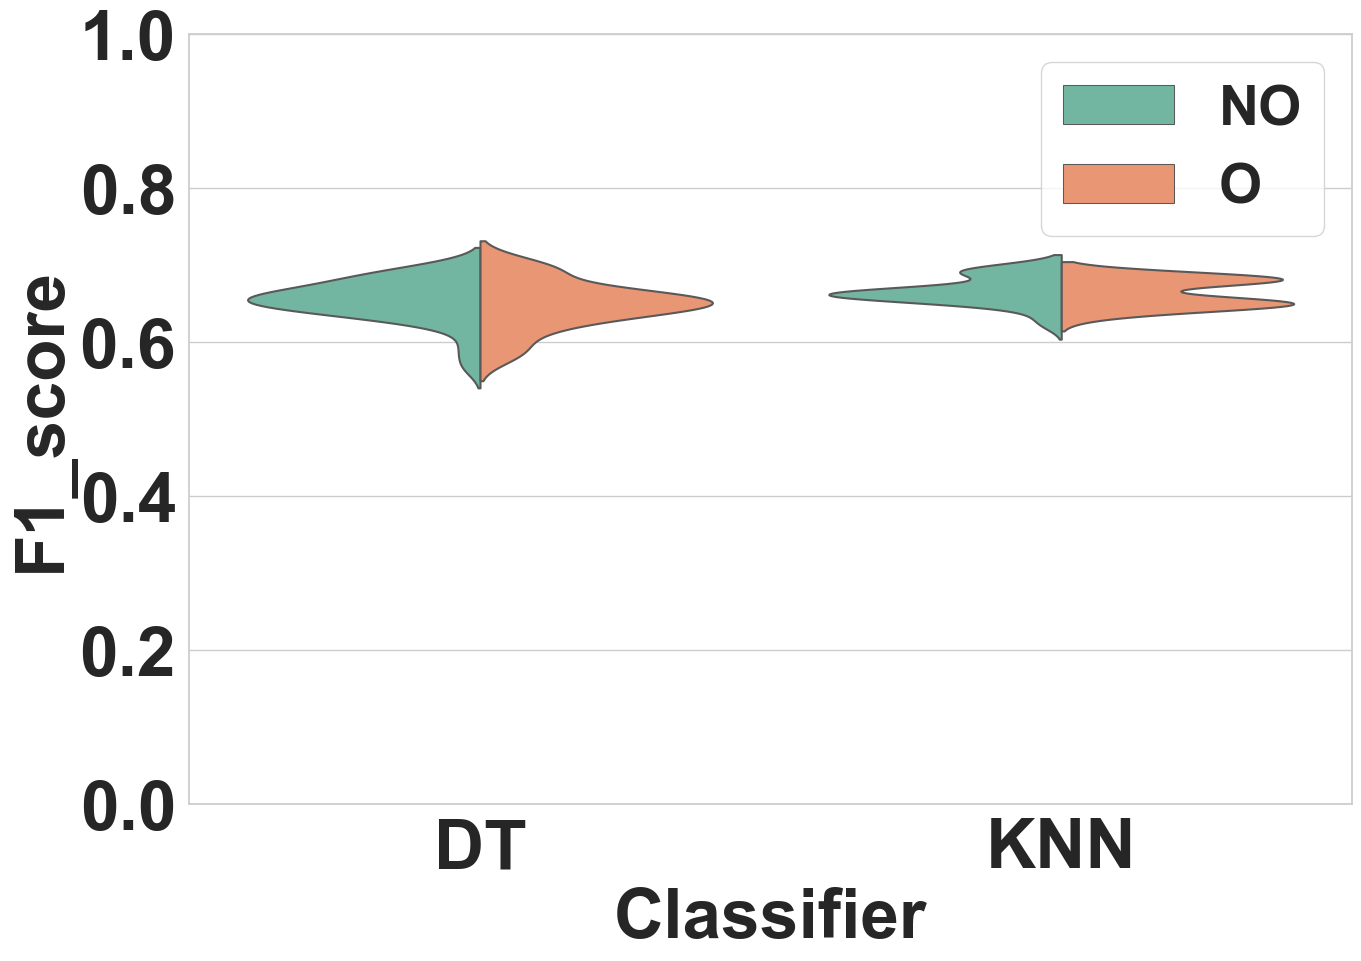
\includegraphics[scale=0.14]{Figures/Dataset2_sbj_FS2_new_hparams.png}}
  \subfigure[FS3]{\label{fig:ds2-FS3-exp3}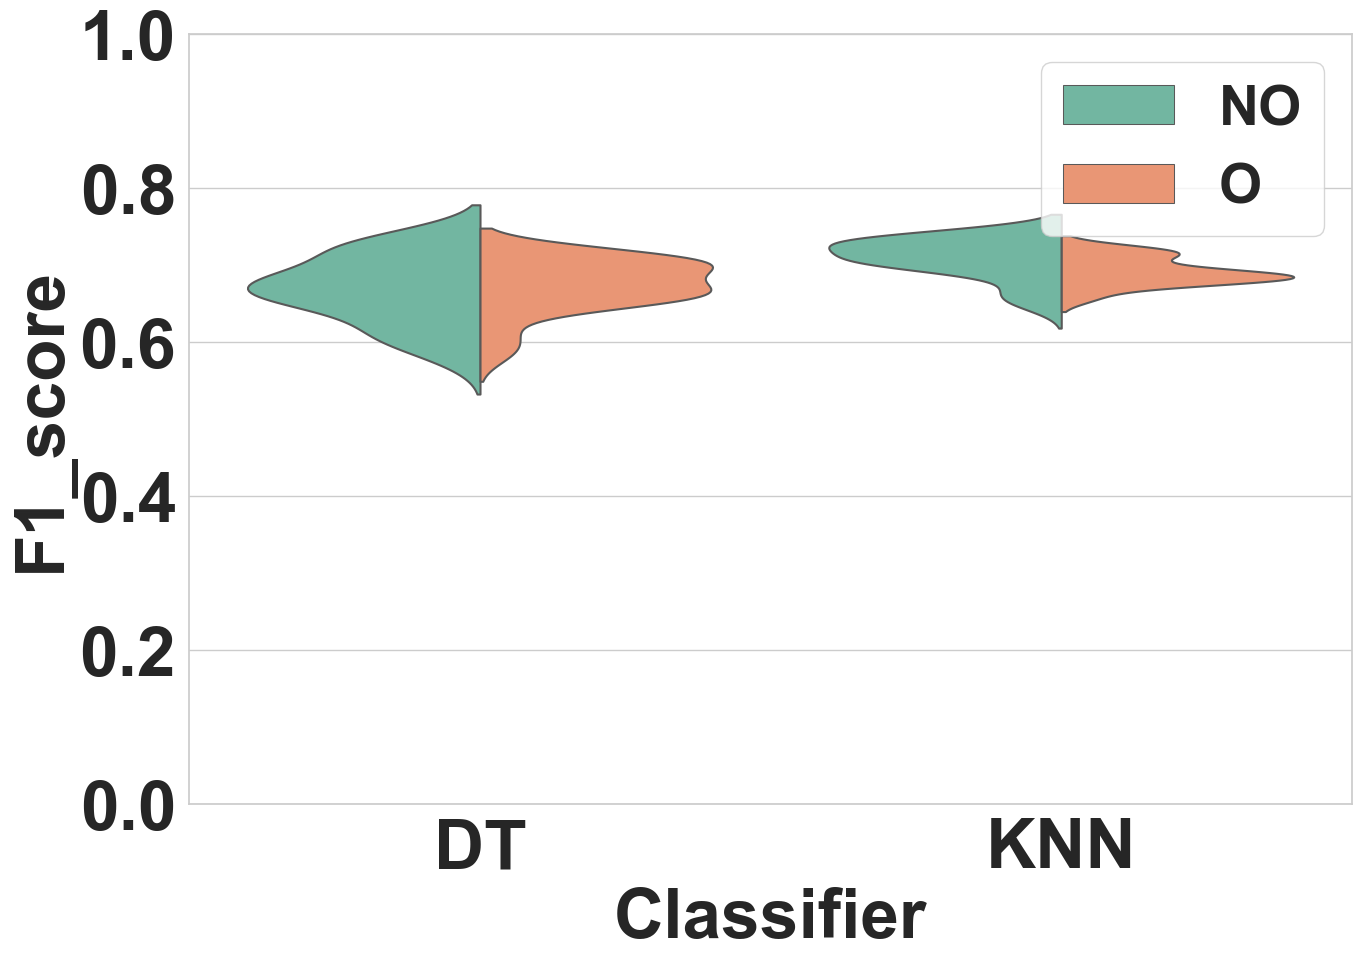
\includegraphics[scale=0.14]{Figures/Dataset2_sbj_FS3_new_hparams.png}}
   
   \caption{Experiment 3 -- Subject-independent CV -- Dataset 2.}
    \label{fig:exp3_ds2}
    
\end{figure}

\section{Activity-Specific evaluation}\label{per_activity_evaluation}
The global evaluation presented previously is useful to have a general view of the effect of windowing techniques in HAR systems. However, it is also interesting to particularize this study to each specific activity. Thus, in this section, we analyze the impact of overlapping and non-overlapping windowing for each activity.

\subsubsection{Experiment 4: Subject-independent CV per activity}
As shown by Experiment 2, overlapping and non-overlapping windowing techniques only lead to minor performance differences when evaluated with subject-independent CV. In this experiment, we investigate how this result particularize to specific activities. The presented data is the same as in Experiment 2, but the classification performance is now detailed for each activity.
For brevity, we only focus on feature set FS3. In all figures, activities are shown with the labels reported in Tables~\ref{tab:Activites1} (Dataset 1) and Tables~\ref{tab:Activites2} (Dataset 2).  

\noindent\textbf{Dataset~1.} In Figure~\ref{fig:exp5_ds1}, the activity-specific F1-scores distributions achieved for all classifiers, window sizes and windowing approaches are presented. As expected from the results shown in~\ref{fig:ds1-FS3-exp2}, the differences between overlapping and non-overlapping windowing for all activities are slow. In general, the performances of the majority of the activities drop (by 5\% on average) when overlapping windowing is used instead of non-overlapping windowing. However, using DT (Figure~\ref{fig:DT_ds1-activity-exp5}), some activities such as Heels  (27), Rotation on knees (30), Trunk Twist (10), Knees (altering) (26), Knees Bending (28), Rowing (31) and Jump rope (8) show a small performance improvement by overlapping windowing.  As for KNN (Figure~\ref{fig:KNN_ds1-activity-exp5}), performance reductions resulting from the use of overlapping windowing are higher than for DT. As an example, using overlapping drops the performance of activity Repetitive forward stretching (17) by 11\%. This may be due to the nature of KNN~\cite{cover1967nearest}, for which a small change in the dataset may have a large impact on the performance. Similar to DT, the performance for some activities also improves when overlapping windows are used, but by less than 2\%. As can be seen in Figure~\ref{fig:NB_ds1-activity-exp5} and Figure~\ref{fig:NCC_ds1-activity-exp5}, the performance of all activities for NB and NCC are almost the same.    



\noindent\textbf{Dataset~2.} Our results for this experiment are shown in Figure~\ref{fig:exp5_ds2}. 

Similar to Dataset~1, the activity-specific F1-score distributions obtained for this dataset for the two scenarios are similar. For this dataset, using overlapping windowing with KNN and DT slightly enhances the F1-score of the majority of activities in comparison to non-overlapping windowing, by 4\% on average. The highest improvements are observed for activities Lawnmower (right) (21), Lateral Raise (19) and Seated Back Fly (31) for DT and for Wall Ball (40), Seated Back Fly (31) and Power Boat pose (26) for KNN. Similar to Dataset~1, the performance of NB and NCC for all activities in both scenarios are almost the same.

This experiment shows that using overlapping windowing with subject-independent validation can impact the recognition performance of HAR systems for diverse activities differently. In spite of being mostly minor, for the activities in this study, overlapping windowing reduces the recognition accuracy of most activities and only a few of them shows improvement. Moreover, the impact of overlapping windowing may be subject to the dataset, i.e., using overlapping windowing may impact the performance of the system in recognizing a single activity in different way. Running is a good example here. Using overlapping windowing reduces the F1-score of the system for this activity in Dataset~1, but it improves that in Dataset~2.  

In summary, the recognition accuracy for most of the activities investigated in this study is quite comparable between the two scenarios with overlapping and non-overlapping windows.    

\subsubsection{Experiment 5: More discriminative features and neural-network classifier}
In this experiment, we evaluate the effectiveness of non-overlapping windows using more discriminative time-domain features and a custom fine-tuned classifier. Namely, we target the HAR framework presented in~\cite{omid2019MPR}. The approach in~\cite{omid2019MPR} utilizes configurable time-domain histogram features and a single hidden layer neural network classifier. It has been shown that the framework can outperform KNN classifiers as well as many other time-domain features explored by previous work. The framework in~\cite{omid2019MPR} allows for a segmentation with a configurable sliding window. It presents results on subject independent cross validation using Dataset~2 and a 5s overlapping window sliding at 200ms steps. Here, we conduct a similar experiment, but with a non-overlapping window size of 5s. To provide a fair comparison, we use the same experimental setup compared to ~\cite{omid2019MPR}, which is presented next. 

We use time-domain histogram features, i.e., 120 bins in total, where 20 bins are assigned uniformly to each individual sensor axis. The accelerometer full-scale range has been set to $\pm{2g}$, while the gyroscope full-scale range has been set to $\pm{512dps}$. The single-hidden-layer neural network classifier consists of 120 input neurons, 60 hidden neurons and 7 output neurons targeting 6 activities and one noise class representing all other activities and the no activity periods. The Sigmoid (Softmax) trigger function has been used for the the hidden (output) layer. Training the neural network has been done in Tensorflow 1.12.0 using a batch size of 32, and the AdamOptimizer algorithm. The number of epochs is chosen, such that the overall number of data points that are fed to the neural network for training becomes identical compared to the experiment in~\cite{omid2019MPR}, i.e., similar training time. 

The normalized confusion matrix for both overlapping and non-overlapping windows under a subject-independent CV process is shown in Table~\ref{tab:MPR Comparison}. The rows refer to the true activities, while the columns correspond to the predicted ones. Each entry in the confusion matrix has two values, where the top value refers to the scenario with overlapping windows, while the bottom value corresponds to the scenario with non-overlapping windows. The results indicate that the use of overlapping windows provides minor improvements on recognition accuracy compared to the non-overlapping windows under subject independent cross validation, even when discriminative features and a well-trained neural network classifier are utilized.

%  start of Table3
\begin{table}
  \centering
\begin{tabular}{|>{}c|>{}c|>{}c|>{}c|>{}c|>{}c|>{}c|>{}c|}
\hline 
Activities & Noise (Others) & Curl & Triceps & Run & Elliptical & JumpJacks & Kettlebell\tabularnewline
\hline 
Noise (Others) & \makecell{\textbf{0.99407} \\ \textbf{0.9928}} & \makecell{0.00094 \\ 0.00103} & \makecell{0.00091 \\ 0.00099} & \makecell{0.00209 \\ 0.00286} & \makecell{0.00127 \\ 0.00129} & \makecell{0.00026 \\ 0.00028} & \makecell{0.00045 \\ 0.00074}\tabularnewline
\hline 
Curl & \makecell{0.1426 \\ 0.1369} & \makecell{\textbf{0.85082} \\ \textbf{0.8492}} & \makecell{0.00659 \\ 0.0139} & \makecell{0 \\ 0} & \makecell{0 \\ 0} & \makecell{0 \\ 0} & \makecell{0 \\ 0}\tabularnewline
\hline
Triceps & \makecell{0.17235 \\ 0.19643} & \makecell{0.00451 \\ 0.00487} & \makecell{\textbf{0.82315} \\ \textbf{0.7987}} & \makecell{0 \\ 0} & \makecell{0 \\ 0} & \makecell{0 \\ 0} & \makecell{0 \\ 0}\tabularnewline
\hline
Run & \makecell{0.20903 \\ 0.20127} & \makecell{0 \\ 0} & \makecell{0 \\ 0} & \makecell{\textbf{0.78668} \\ \textbf{0.79237}} & \makecell{0.00429 \\ 0.00565} & \makecell{0 \\ 0} & \makecell{0 \\ 0.00071}\tabularnewline
\hline
Elliptical & \makecell{0.16742 \\ 0.16265} & \makecell{0 \\ 0} & \makecell{0 \\ 0} & \makecell{0.00916 \\ 0.03113} & \makecell{\textbf{0.82342} \\ \textbf{0.80622}} & \makecell{0 \\ 0} & \makecell{0 \\ 0}\tabularnewline
\hline
JumpJacks & \makecell{0.20147 \\ 0.23729} & \makecell{0 \\ 0} & \makecell{0 \\ 0} & \makecell{0 \\ 0} & \makecell{0 \\ 0} & \makecell{\textbf{0.79853} \\ \textbf{0.76271}} & \makecell{0 \\ 0}\tabularnewline
\hline
Kettlebell & \makecell{0.18938 \\ 0.21484} & \makecell{0.00287 \\ 0} & \makecell{0 \\ 0} & \makecell{0 \\ 0} & \makecell{0 \\ 0} & \makecell{0 \\ 0} & \makecell{\textbf{0.80775} \\ \textbf{0.78516}}\tabularnewline
\hline
\end{tabular}
    \caption{Normalized confusion matrix for Experiment 5, i.e., six activities and one noise class representing all other activities and no activity periods from Dataset 2 under subject independent cross validation. Rows are true activities, and columns are predicted ones. Each entry has two values, where the top (bottom) value refers to the scenario with overlapping (non-overlapping) windows.}
    \label{tab:MPR Comparison}
\end{table}

\begin{figure}[htp]
  \centering
  \subfigure[DT]{\label{fig:DT_ds1-activity-exp5}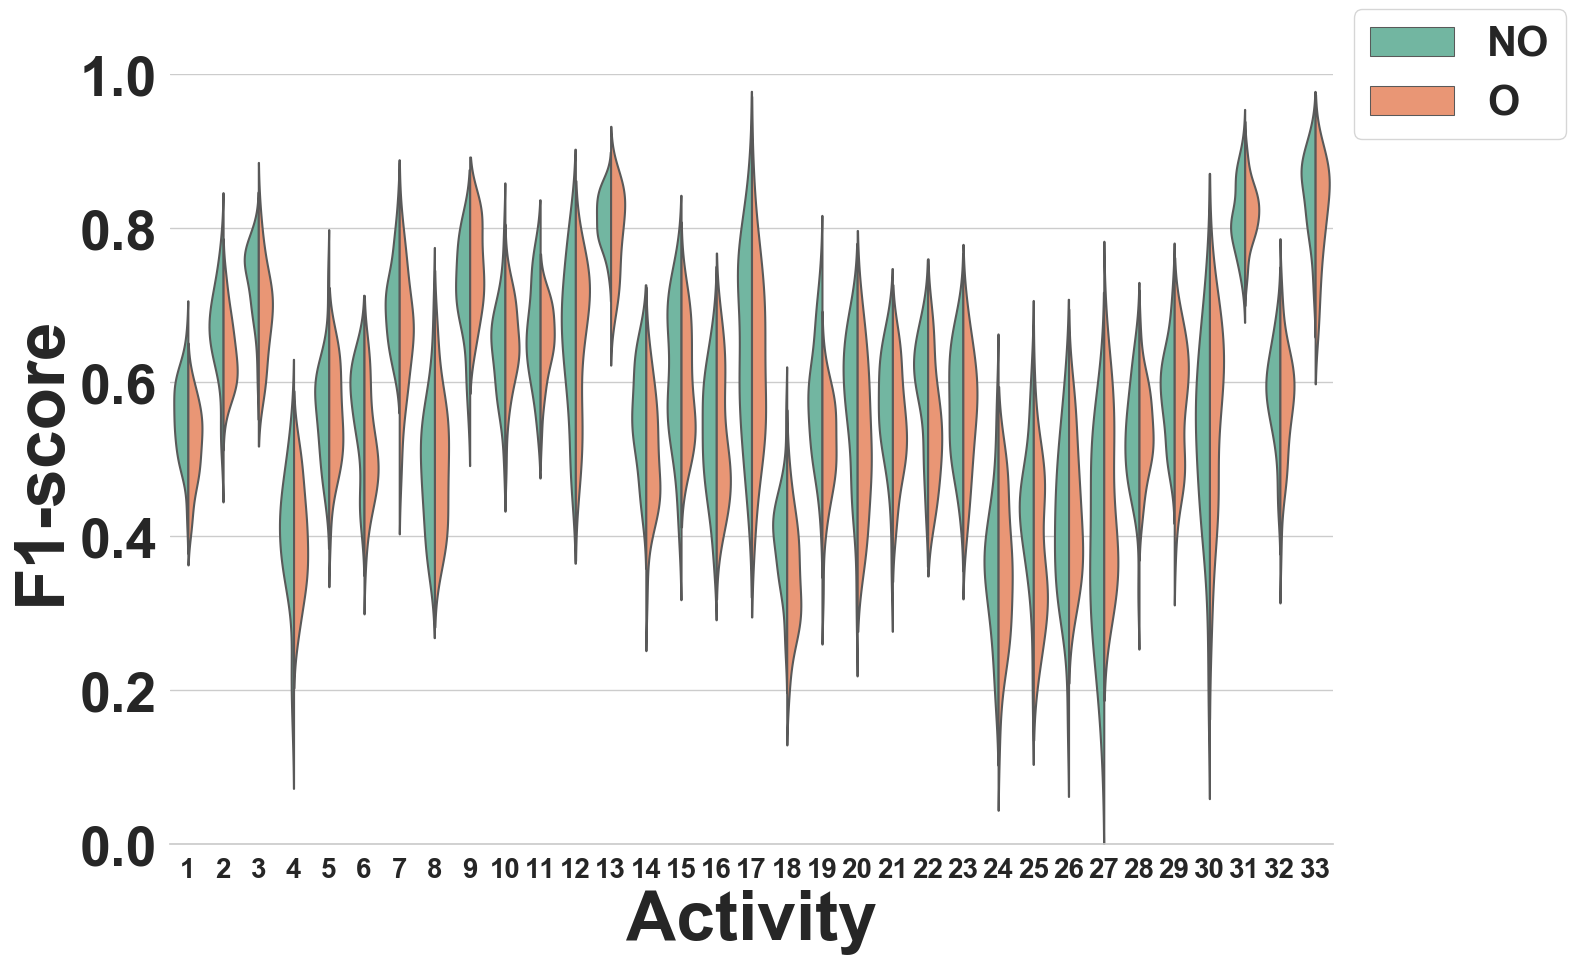
\includegraphics[scale=0.18]{Figures/per_activity_Dataset1_DT_sbj_FS3.png}}\quad
  \subfigure[KNN]{\label{fig:KNN_ds1-activity-exp5}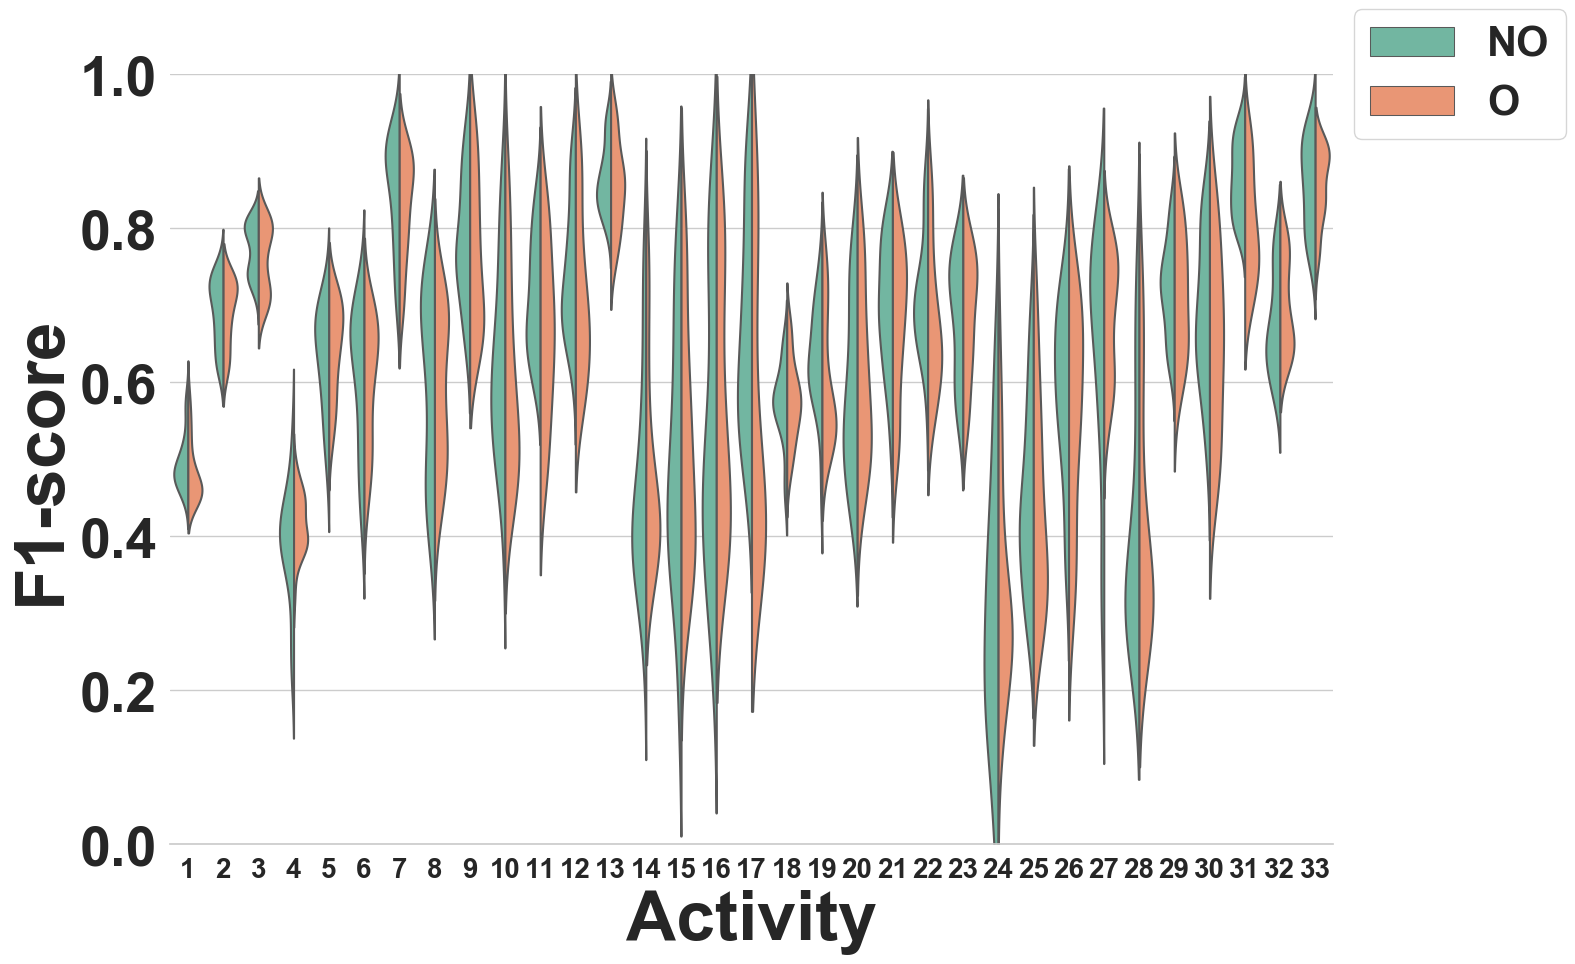
\includegraphics[scale=0.18]{Figures/per_activity_Dataset1_KNN_sbj_FS3.png}}
  \subfigure[NB]{\label{fig:NB_ds1-activity-exp5}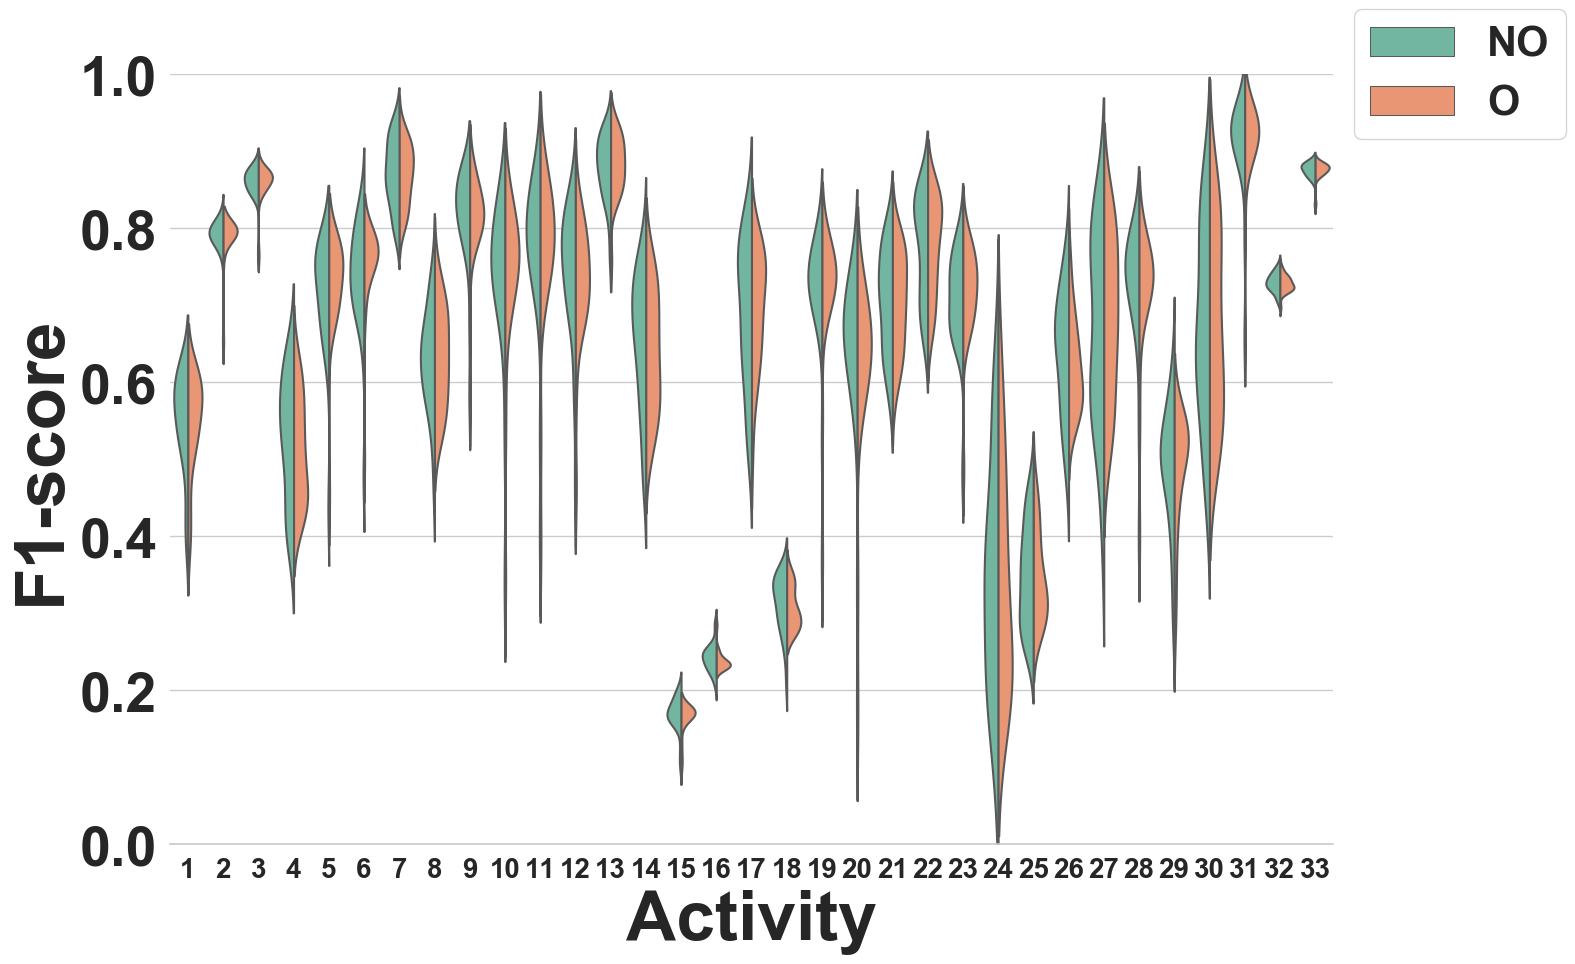
\includegraphics[scale=0.18]{Figures/per_activity_Dataset1_NB_sbj_FS3.png}}
    \subfigure[NCC]{\label{fig:NCC_ds1-activity-exp5}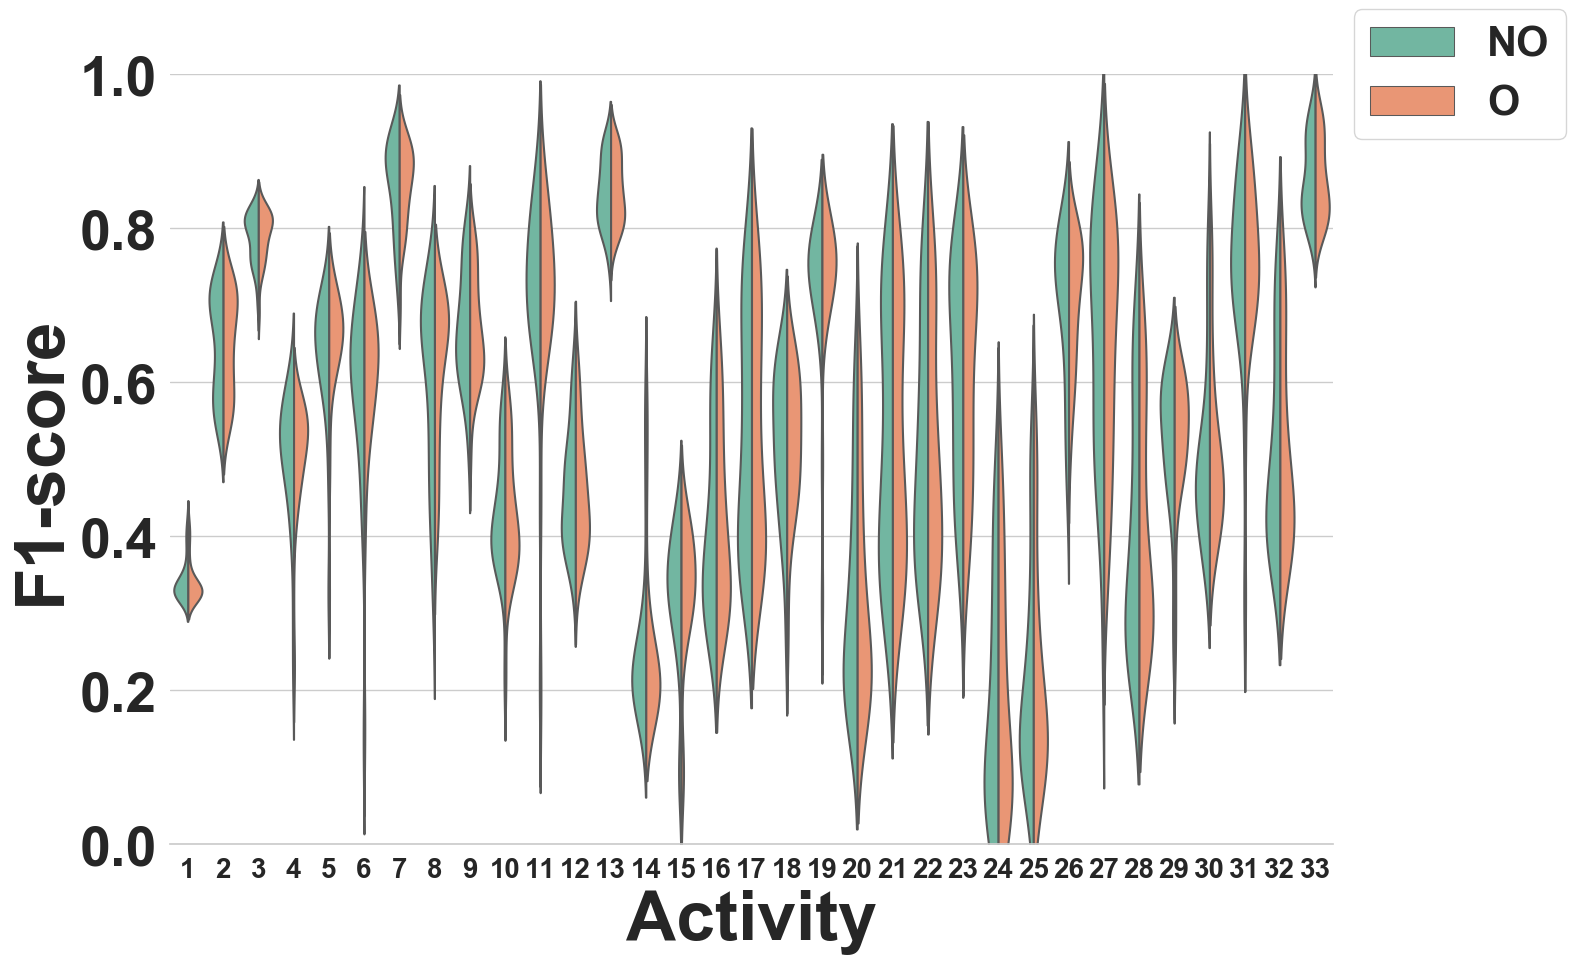
\includegraphics[scale=0.18]{Figures/per_activity_Dataset1_NCC_sbj_FS3.png}}
   
   \caption{Experiment 4 -- Subject-independent CV -- Dataset 1.}
    \label{fig:exp5_ds1}
    
\end{figure}

\begin{figure}[htp]
  \centering
  \subfigure[DT]{\label{fig:DT_ds2-activity-exp5}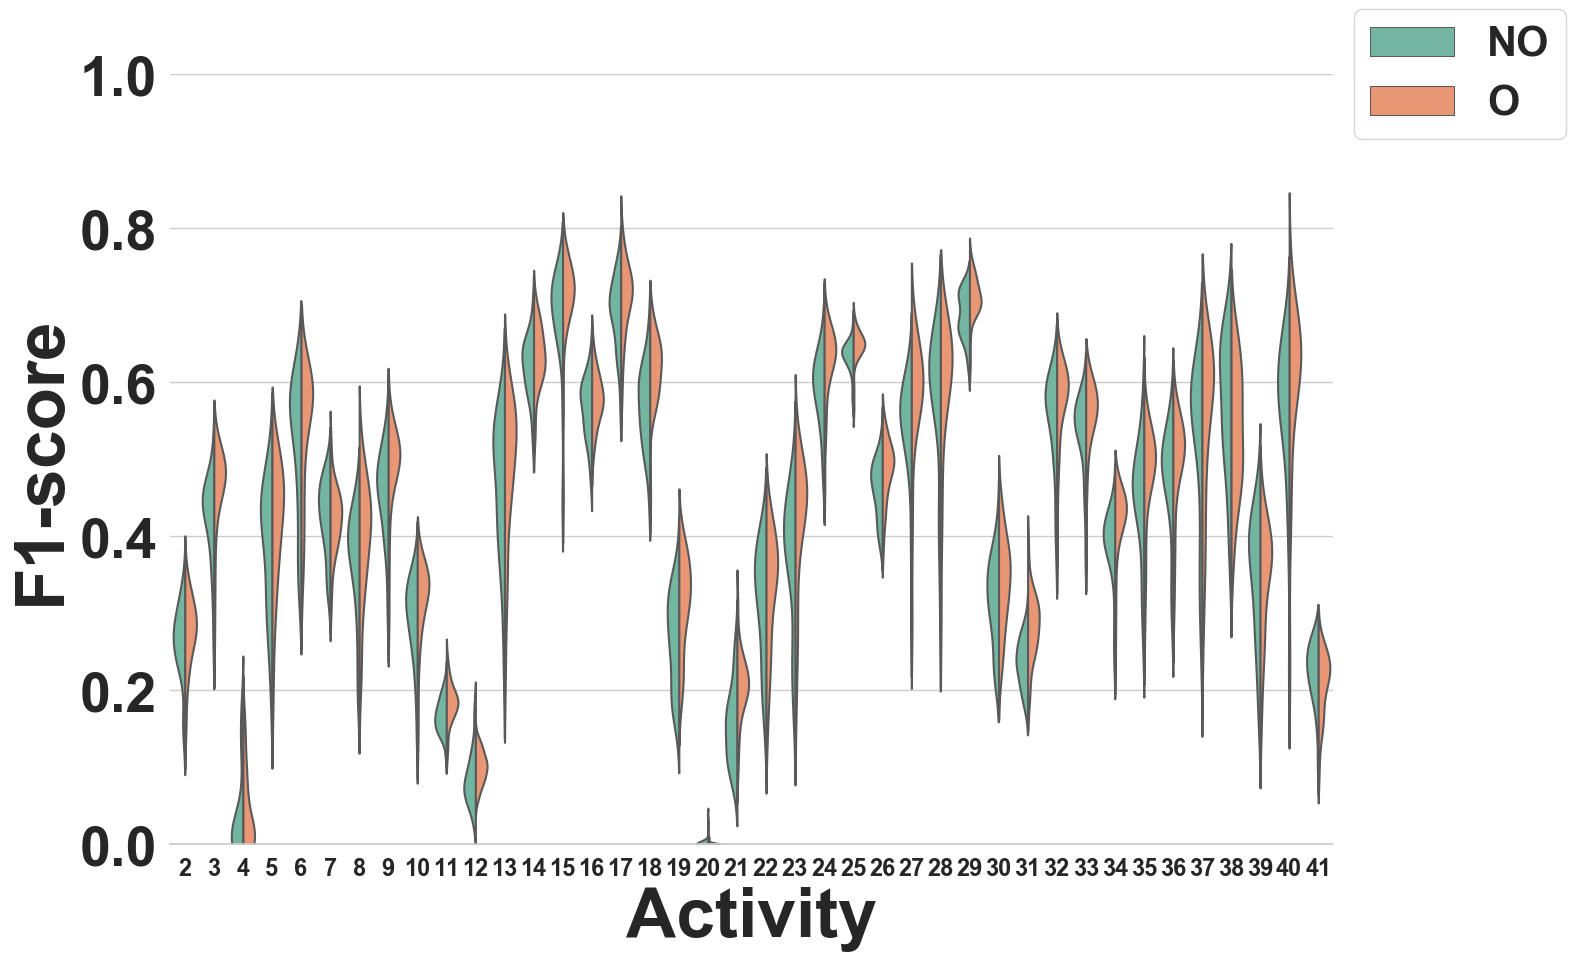
\includegraphics[scale=0.18]{Figures/per_activity_Dataset2_DT_sbj_FS3.png}}\quad
  \subfigure[KNN]{\label{fig:KNN_ds2-activity-exp5}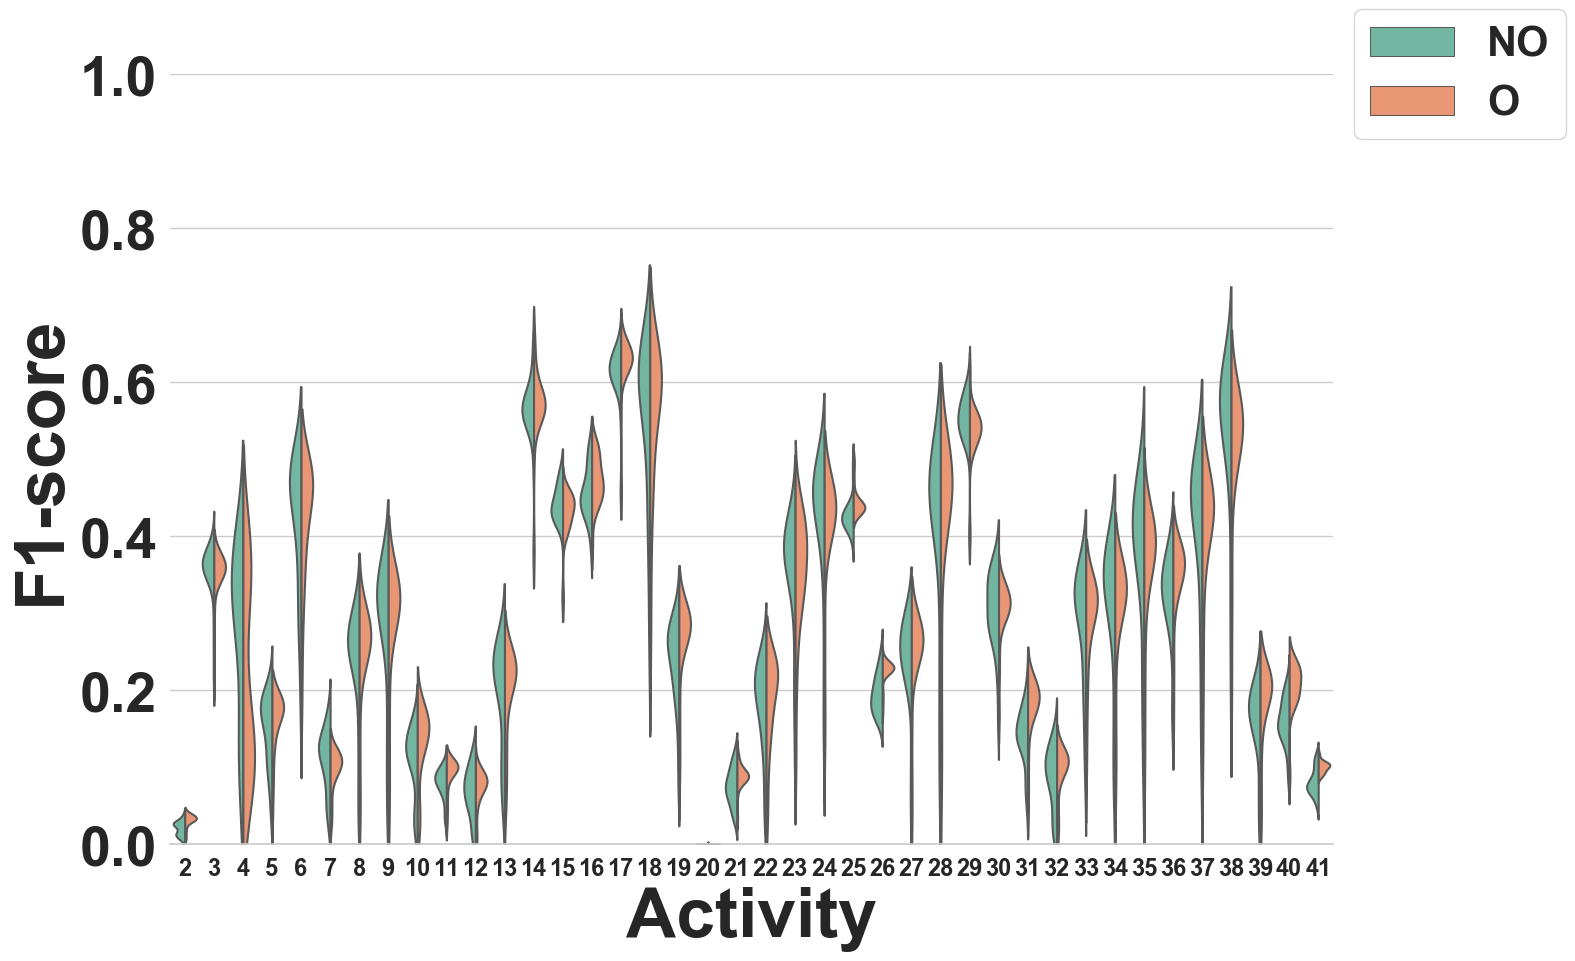
\includegraphics[scale=0.18]{Figures/per_activity_Dataset2_KNN_sbj_FS3.png}}
  \subfigure[NB]{\label{fig:NB_ds2-activity-exp3}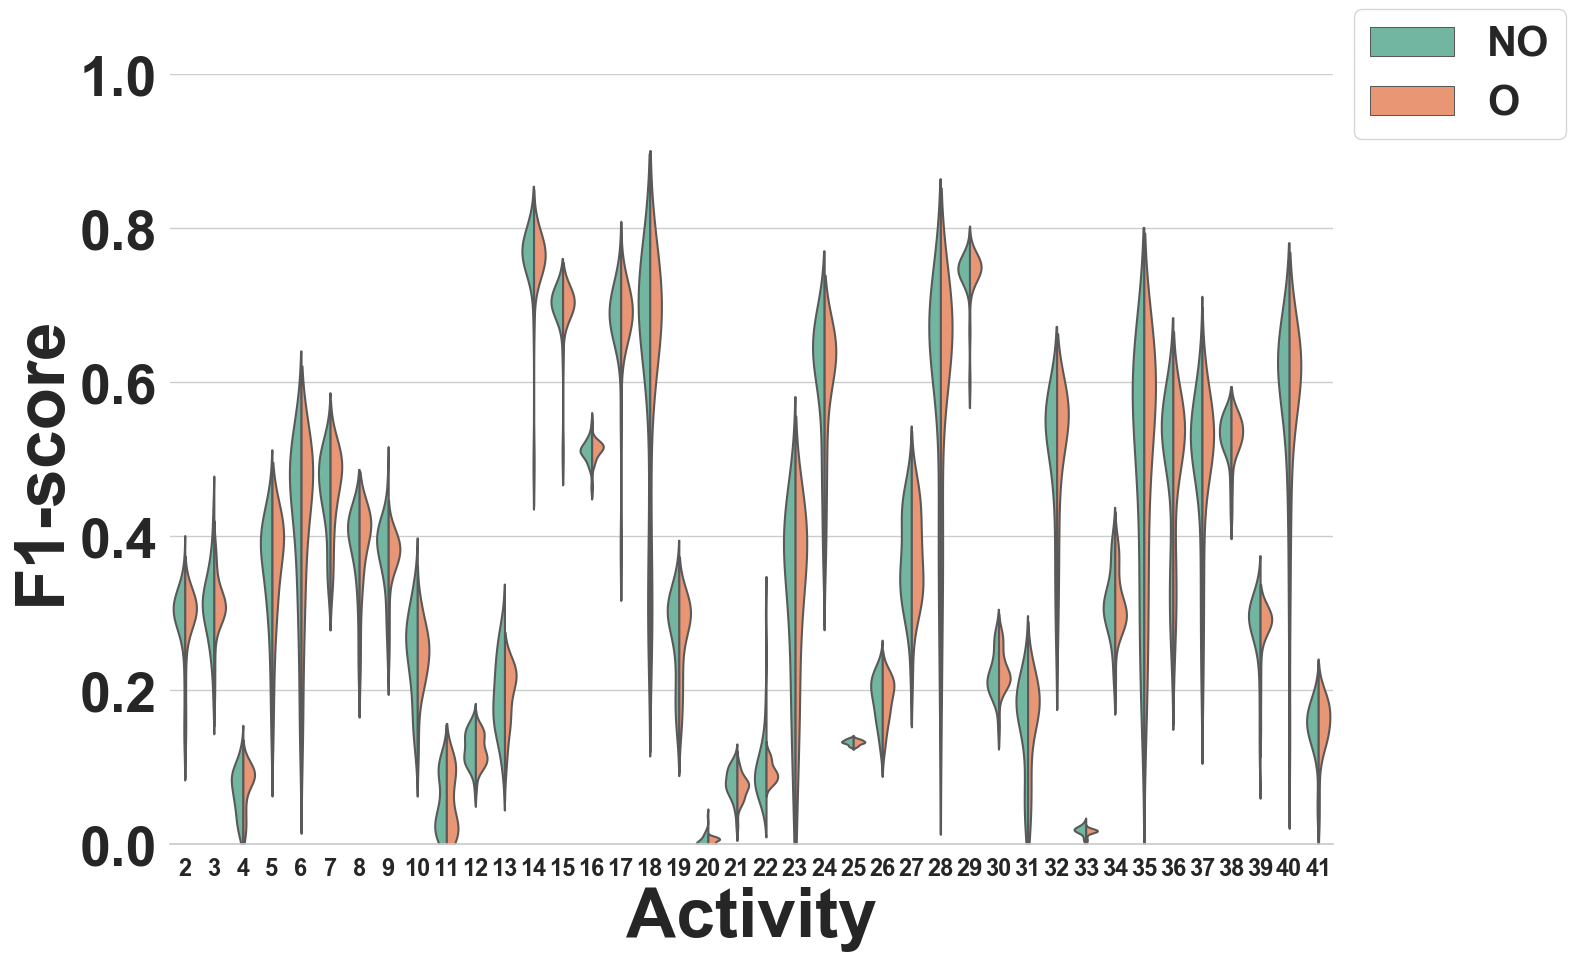
\includegraphics[scale=0.18]{Figures/per_activity_Dataset2_NB_sbj_FS3}}
    \subfigure[NCC]{\label{fig:NCC_ds2-activity-exp5}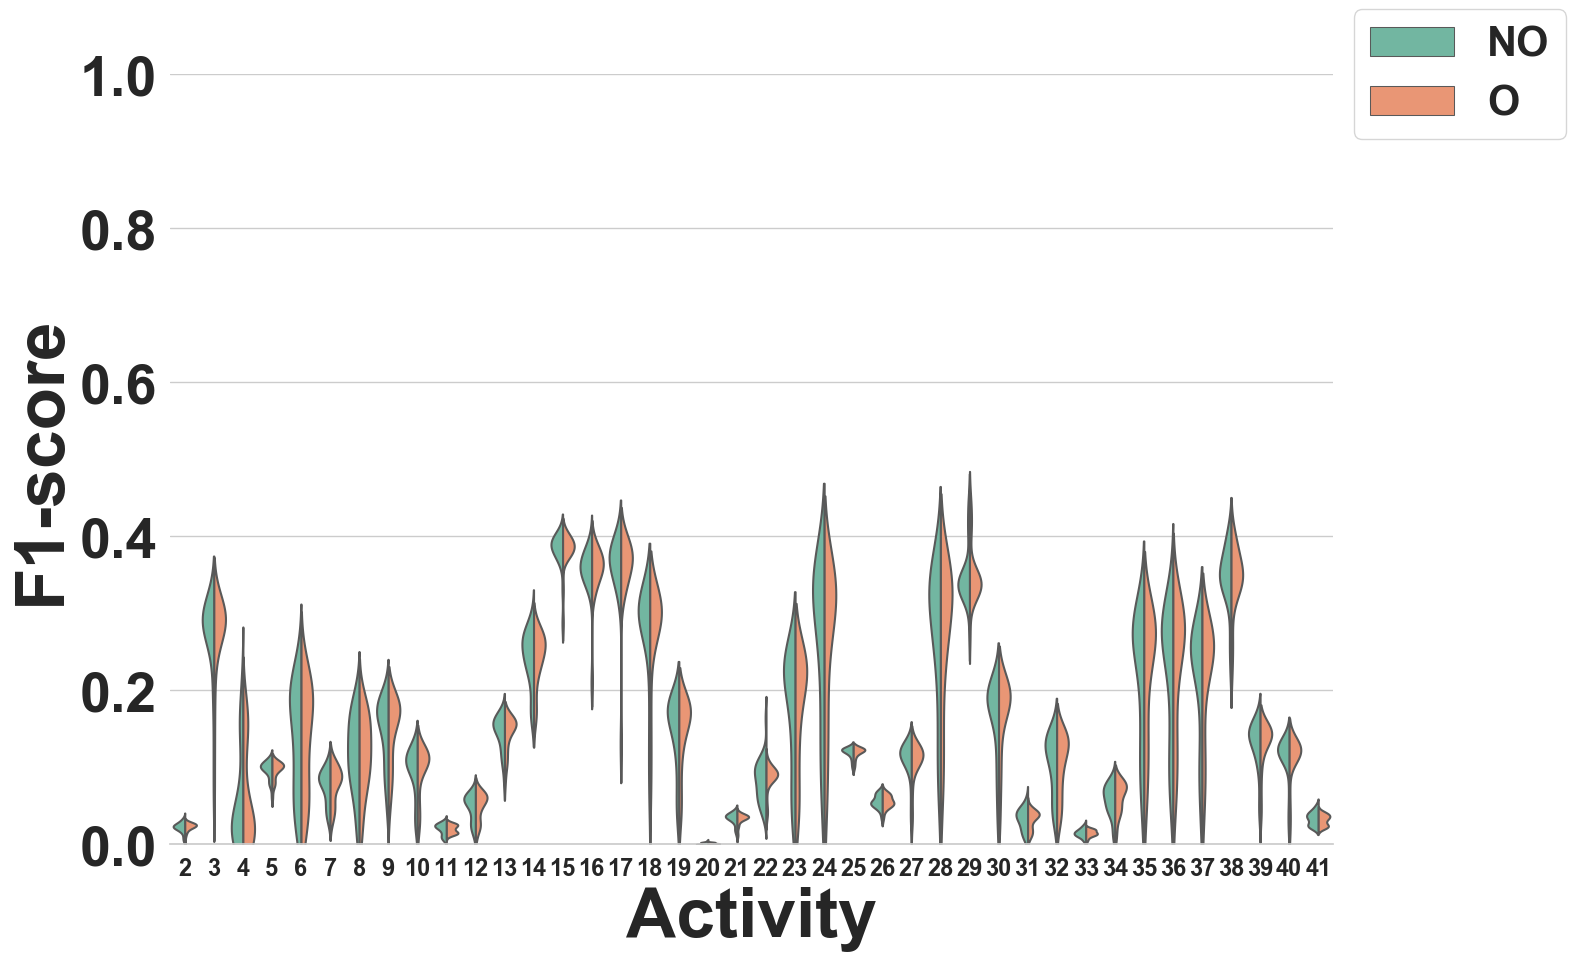
\includegraphics[scale=0.18]{Figures/per_activity_Dataset2_NCC_sbj_FS3.png}}
   
   \caption{Experiment 4 -- Subject-independent CV -- Dataset 2.}
    \label{fig:exp5_ds2}
    
\end{figure}

\chapter{Discussion and conclusion} \label{discussion_conclusion}
\section{Discussion} \label{sec:discussion}
% Compare the nonoverlapping in sbj dependent and independent CVs
As can be seen by comparing the results of Experiment 1 and 2 for non-overlapping windowing, using Subject independent CV instead of 
Subject-dependent CV reduces the F1-score of KNN and DT by 10\% and 11\% on average for Dataset 1 and 2 respectively, which is substantial. It confirms that samples drawn from the 
same subject cannot be considered independent. In an ARP setup, Subject dependent CV overestimates the classification performance and should, therefore, be avoided.
% Compare the overlapping in sbj dependent and independent CVs
The detrimental effect of subject-dependent CV is even larger when overlapping time windows are used. In this case, as can be seen by comparing the results of Experiment 1 and 2 for overlapping windowing, Subject-independent CV reduces the F1-score of KNN and DT by 16\% and 21\% on average for Dataset 1 and 2 respectively. This 
further confirms that within-subject dependencies between time windows account for a significant part of the performance measured through 
Subject-dependent CV. Furthermore, for overlapping windows, the performance 
difference between subject-dependent CV and subject independent CV increases with the window 
size. This is consistent with our previous comments, as the amount of 
overlap between overlapping windows, and therefore their correlation, 
also increases with the window size.
% Overlapping windowing is not important once comes with sbj independent

Comparing the results for overlapping and non-overlapping windowing in Figure~\ref{fig:exp1_ds1} and Figure~\ref{fig:exp1_ds2} shows that when using Subject-dependent CV, overlapping windowing can improve the recognition power of the classifiers, which coincides with the general idea that overlapping windowing improves the performance of HAR systems~\cite{janidarmian2017comprehensive,janidarmian2014automated}. 
However, our results confirm that such improvement comes from the 
increasing correlation among test and train folds due to the underlying 
problems of Subject-dependent CV in HAR systems.      
% Overlapping windowing is not important once comes with sbj independent
In contrast, when using Subject independent CV, the impact of using overlapping
windows is minor to negligible, as can be seen in  
Figure~\ref{fig:exp2_ds1} and Figure~\ref{fig:exp2_ds2}. This is in contradiction with 
the common argument that overlapping windows improve classification
performance by bringing more data to the classifier. However, it also 
confirms our hypothesis that the performance increase coming from 
overlapping windows is, in fact, coming from the extra correlation 
between time windows, when Subject-dependent CV is used.

Experiment~3 showed that this conclusion also holds when using a different set of hyperparameters, which improves the generalizability of our result. 

The results of Experiment 4 show that the impact of overlapping windowing with subject independent CV can be different per activity. In other words, overlapping windowing for some activities such as Trunk Twist and Lateral Raise improves the recognition performances and for others like Repetitive forward stretching and Heels not. However, such changes remain negligible for most activities and using this technique in HAR seems to be non-beneficial. 

Experiment 5 explored the use of more discriminative features with a neural-network model, and the results similarly suggest that the use of overlapping windows does not provide major performance improvements.


Finally, Table~\ref{tab:resources} shows the data size and required time for segmentation and training in overlapping and non-overlapping windowing techniques with subject independent CV for two datasets. Segmenting using overlapping windows is almost twice longer than with non-overlapping windows, which is significant. Similarly, training on the data windowed by overlapping windows technique takes 4 times of non-overlapping one. As for storage, the size of segmented data by overlapping sliding windows technique is almost 9 times of data produced by non-overlapping one for both datasets. In spite of such increase in size and computation, this technique does not improve the performance of the classifiers when used with Subject independent CV.

%The resource issues are even worse in active learning


% we use the dataset of two wellknown HAR database which contain different type of activities ranging from ....... .  Having such big distributin of activites help us to be confident about our results.

\begin{table}[]
\begin{tabular}{|c|c|>{\centering}m{1.5cm}|c|>{\centering}m{1.5cm}|c|c|c|}
\hline 
\multirow{2}{*}{Dataset} & \multirow{2}{*}{Raw size (GB)} & \multicolumn{3}{c|}{Nonoverlapping windowing} & \multicolumn{3}{c|}{Overlapping windowing }\tabularnewline
\cline{3-8} \cline{4-8} \cline{5-8} \cline{6-8} \cline{7-8} \cline{8-8} 
 &  & \multicolumn{2}{c|}{Segmentation } & \multirow{2}{1.5cm}{Training time (day)} & \multicolumn{2}{c|}{Segmentation } & \multirow{2}{*}{Training time (day)}\tabularnewline
\cline{1-4} \cline{2-4} \cline{3-4} \cline{4-4} \cline{6-7} \cline{7-7} 
\multicolumn{1}{c}{-} & - & Time (Hour) & Size(GB) &  & Time (Hour) & Size (GB) & \tabularnewline
\hline 
1 & 2.4 & 6.0 & 2.3 & 1.0 & 11.0 & 21 & 4.0\tabularnewline
\hline 
2 & 3.4 & 12.0 & 5.8 & 2.0 & 20.0 & 51 & 8.0\tabularnewline
\hline 
\end{tabular}
        \caption{Overlapping windowing vs. nonoverlapping windowing required resources - Subject independent CV}
        \label{tab:resources}
\end{table}

\section{Conclusion} \label{sec:conclusion}
We conclude that the suggested use of overlapping sliding windows in HAR systems is associated with underlying limitations of subject-dependent CV. When subject-independent CV is used, overlapping sliding windows do not improve the performance of HAR systems but still require substantially more resources than non-overlapping windows.


Our results show that the performance of all classifiers drops when subject-independent CV is used rather than subject-dependent CV. One possible way to address this problem would be to use features that are more common among subjects with different characteristics. Thus,   
in our future work, we will design such features and investigate their impact on the performance of HAR systems. This would enable building more generalized systems with a limited number of subjects. 

%\include{Experiment} % chapter title as the chapter name.


%%%%%%%%%% Appendices %%%%%%%%%%%%%%%%
% ---- Appendix settings. Please Do NOT change them. -----
\appendix
\setcounter{table}{0}		% reset the table counter
\setcounter{figure}{0}		% reset the figure counter
\renewcommand{\thefigure}{\Alph{chapter}.\arabic{figure}} 	% numbering the a figure in Appendix as Figure A.2, Figure B.1, etc.
\renewcommand{\thetable}{\Alph{chapter}.\arabic{table}}		% numbering the a table in Appendix as Table A.2, Table B.1, etc.

%%%%%%%%%% Body of Appendix %%%%%%%%%%%%%%%%
\begin{appendices}
    %\chapter{My Appendix} \label{chap:ApdxA}

Appendix figure example is shown in \ref{fig:encslogo} below
 
 %%%%%%%%%%%%%%%% begin figure %%%%%%%%%%%%%%%%%%%
 \begin{figure}[htp]
     \begin{center}
         
\includegraphics[scale=0.5]{ENCSlogo}  %it is suggested to using scale to zoom figures without distortion
        \end{center}
        \caption{An figure example in Appendix \ref{chap:ApdxA}.}
        \label{fig:encslogo}
    \end{figure}
%%%%%%%%%%%%%%%% end figure %%%%%%%%%%%%%%%%%%%
    
    

    %\include{Appendix_B}
\end{appendices}





%%%%%%%%%% References %%%%%%%%%%%%%%%%%
\addcontentsline{toc}{chapter}{Bibliography}
 %  Add Bibliography to TOC
\bibliography{ThesisRef.bib}
\bibliographystyle{unsrt}
% Your .bib files name here
 	% References are in APA style
\setcitestyle{square}
\end{document}
